\section{Literature review}\label{sec:lit_review}

This chapter presents a review of the research landscape surrounding the topics discussed in the introduction. In Section~\ref{lr-vbds}, I discuss vector-borne diseases (VBDs) and behavioural tendencies for adopting measures of self-protection. In Section~\ref{lr-abm}, I introduce traditional methods for modelling VBDs and I motivate the agent-based approach used in this research, before concluding with an assessment of techniques for representing preventive behaviours in agent-based models (ABMs).

%vector-borne diseases (VBDs), behavioural attitudes for preventive measures, and mathematical and computational approaches to modelling VBDs. First, I present an epidemiological background of VBDs and discuss behavioural tendencies for adopting measures for self-protection. Second, I cover traditional methods for modelling VBDs and I motivate the agent-based approach, before concluding with modern approaches to representing preventive behaviours in ABMs.


\subsection{Vector-borne diseases}\label{lr-vbds}

VBDs are infectious diseases transmitted by \textit{vectors}---living organisms that enable human-human or animal-human transmission of infectious pathogens. Examples of VBDs include malaria and dengue, transmitted by mosquitoes, and leishmaniasis, transmitted by sandflies \cite{world_health_organisation_who_vector-borne_2020}. Not only do these diseases put pressure on public health systems with over one billion infections every year \cite{world_health_organisation_who_global_2004}, but they also increase health inequalities and hinder socioeconomic growth in underdeveloped nations that have tropical climates or insufficient coverage of health services \cite{campbell-lendrum_climate_2015}.

\begin{figure}[h]
\centering

\begin{tikzpicture}[node distance=1cm, auto,
                >=Latex, 
                every node/.append style={align=center, font=\small},
                int/.style={draw, thick}]

\newcommand{\drawagentat}[4]{
    \tikzset{shift={(#1,#2)}}
    
    \path[draw=black,fill=#3,miter limit=10.0,scale=#4] (1.6431, -0.2275).. controls (1.5055, -0.2275) and (1.3944, -0.3387) .. (1.3944, -0.4763).. controls (1.3944, -0.6138) and (1.5055, -0.725) .. (1.6431, -0.725).. controls (1.7806, -0.725) and (1.8918, -0.6138) .. (1.8918, -0.4763).. controls (1.8918, -0.3387) and (1.7806, -0.2275) .. (1.6431, -0.2275) -- cycle(1.3679, -0.7911).. controls (1.1906, -0.7911) and (1.0478, -0.934) .. (1.0478, -1.1113) -- (1.0478, -1.8838).. controls (1.0478, -1.9447) and (1.0954, -1.9923) .. (1.1562, -1.9923).. controls (1.2171, -1.9923) and (1.2647, -1.9447) .. (1.2647, -1.8838) -- (1.2647, -1.1853) -- (1.3203, -1.1853).. controls (1.3203, -1.1853) and (1.3203, -3.0057) .. (1.3203, -3.1247).. controls (1.3203, -3.2041) and (1.3864, -3.2703) .. (1.4658, -3.2703).. controls (1.5478, -3.2703) and (1.6113, -3.2041) .. (1.6113, -3.1247) -- (1.6113, -1.9976) -- (1.6722, -1.9976) -- (1.6722, -3.1247).. controls (1.6722, -3.2041) and (1.7383, -3.2703) .. (1.8177, -3.2703).. controls (1.8997, -3.2703) and (1.9632, -3.2041) .. (1.9632, -3.1247) -- (1.9632, -1.1853) -- (2.0188, -1.1853) -- (2.0188, -1.8838).. controls (2.0188, -1.9447) and (2.0664, -1.9923) .. (2.1273, -1.9923).. controls (2.1881, -1.9923) and (2.2357, -1.9447) .. (2.2357, -1.8838) -- (2.2357, -1.1086).. controls (2.2357, -0.9313) and (2.0902, -0.7885) .. (1.9156, -0.7885).. controls (1.9182, -0.7911) and (1.3679, -0.7911) .. (1.3679, -0.7911) -- cycle;

    \tikzset{shift={(-#1,-#2)}}
    }

\newcommand{\drawmosquitoat}[3]{
    \tikzset{shift={(#1,#2)}}

    \path[draw=black,fill=#3,miter limit=10.0,line width=0.0001cm,scale=.5] (1.5779, -0.1786).. controls (1.5669, -0.1812) and (1.5472, -0.1912) .. (1.5356, -0.1999).. controls (1.4706, -0.2489) and (1.4023, -0.3617) .. (1.3047, -0.5818) -- (1.2865, -0.6227) -- (1.2778, -0.6065).. controls (1.2549, -0.5642) and (1.2251, -0.5267) .. (1.1826, -0.4866).. controls (1.1259, -0.4332) and (1.1002, -0.4158) .. (1.0708, -0.411).. controls (1.0548, -0.4083) and (1.0384, -0.4131) .. (1.0244, -0.4245).. controls (1.0177, -0.4299) and (1.0057, -0.4453) .. (0.9996, -0.4566).. controls (0.9873, -0.4783) and (0.9739, -0.5204) .. (0.9651, -0.5645).. controls (0.9486, -0.6463) and (0.939, -0.7409) .. (0.9265, -0.9452).. controls (0.9241, -0.9832) and (0.9232, -1.1225) .. (0.925, -1.173).. controls (0.9279, -1.2566) and (0.9328, -1.3343) .. (0.9423, -1.4448).. controls (0.9449, -1.4755) and (0.9471, -1.5021) .. (0.9471, -1.5041).. controls (0.9471, -1.5074) and (0.9464, -1.508) .. (0.942, -1.5087).. controls (0.9095, -1.5139) and (0.8738, -1.5243) .. (0.8494, -1.5358).. controls (0.7839, -1.5665) and (0.7361, -1.6163) .. (0.715, -1.6761).. controls (0.711, -1.6871) and (0.7099, -1.6882) .. (0.7055, -1.6845).. controls (0.7007, -1.6805) and (0.6862, -1.6726) .. (0.676, -1.6685).. controls (0.5991, -1.6377) and (0.5126, -1.6836) .. (0.4672, -1.7791).. controls (0.4606, -1.7928) and (0.4511, -1.8196) .. (0.4474, -1.8343) -- (0.4459, -1.8401) -- (0.4319, -1.8353).. controls (0.3542, -1.8082) and (0.2813, -1.7632) .. (0.2143, -1.7006) -- (0.1987, -1.686) -- (0.1785, -1.7062) -- (0.1582, -1.7265) -- (0.1747, -1.7422).. controls (0.2473, -1.8116) and (0.3334, -1.8639) .. (0.423, -1.8932) -- (0.4392, -1.8984) -- (0.4399, -1.9033).. controls (0.4403, -1.906) and (0.4414, -1.9127) .. (0.4424, -1.9182).. controls (0.4433, -1.9237) and (0.4439, -1.9285) .. (0.4435, -1.9286).. controls (0.4419, -1.9296) and (0.4016, -1.9362) .. (0.3884, -1.9377).. controls (0.3537, -1.9416) and (0.2951, -1.9416) .. (0.2574, -1.9377).. controls (0.237, -1.9355) and (0.2109, -1.9312) .. (0.1889, -1.9267).. controls (0.1782, -1.9245) and (0.1692, -1.9231) .. (0.1686, -1.9237).. controls (0.1682, -1.9242) and (0.1652, -1.9357) .. (0.162, -1.9493).. controls (0.1587, -1.9629) and (0.1559, -1.975) .. (0.1556, -1.9762).. controls (0.155, -1.978) and (0.1585, -1.9793) .. (0.1747, -1.9827).. controls (0.243, -1.9975) and (0.3129, -2.0023) .. (0.3788, -1.9966).. controls (0.4038, -1.9944) and (0.4509, -1.9871) .. (0.4628, -1.9835).. controls (0.4646, -1.983) and (0.4661, -1.9846) .. (0.4684, -1.9894).. controls (0.4776, -2.0074) and (0.5007, -2.0393) .. (0.5224, -2.0641) -- (0.5364, -2.08) -- (0.4775, -2.5068).. controls (0.4113, -2.9862) and (0.4163, -2.9414) .. (0.4274, -2.9532).. controls (0.441, -2.9675) and (0.465, -2.964) .. (0.4732, -2.9464).. controls (0.4752, -2.9424) and (0.5019, -2.8017) .. (0.5545, -2.5211).. controls (0.5976, -2.2905) and (0.6332, -2.1008) .. (0.6336, -2.0995).. controls (0.6339, -2.0983) and (0.6395, -2.094) .. (0.6459, -2.09).. controls (0.6794, -2.0695) and (0.7143, -2.0409) .. (0.7365, -2.0158).. controls (0.7651, -1.9835) and (0.7814, -1.9521) .. (0.7869, -1.9195) -- (0.7886, -1.909) -- (0.7961, -1.9149).. controls (0.8149, -1.9296) and (0.8453, -1.9462) .. (0.8723, -1.9562).. controls (0.8863, -1.9614) and (0.9164, -1.9695) .. (0.9283, -1.9713).. controls (0.9319, -1.9718) and (0.9348, -1.9727) .. (0.9348, -1.9732).. controls (0.9348, -1.9737) and (0.8922, -1.9996) .. (0.8403, -2.0307) -- (0.7459, -2.0874) -- (0.7468, -2.0959).. controls (0.7474, -2.1006) and (0.7628, -2.2306) .. (0.781, -2.3846) -- (0.8142, -2.665) -- (0.7426, -2.7558).. controls (0.6836, -2.8308) and (0.6712, -2.8471) .. (0.6728, -2.8485).. controls (0.6799, -2.8551) and (0.7155, -2.882) .. (0.7165, -2.8814).. controls (0.7172, -2.881) and (0.753, -2.8359) .. (0.7961, -2.7812) -- (0.8745, -2.6817) -- (0.8414, -2.4034).. controls (0.8233, -2.2502) and (0.8083, -2.1234) .. (0.8081, -2.1213).. controls (0.8078, -2.1178) and (0.8129, -2.1145) .. (0.9173, -2.0519) -- (1.0268, -1.9861) -- (1.0268, -2.0117) -- (1.0268, -2.0372) -- (0.9308, -2.1333) -- (0.8348, -2.2294) -- (0.9377, -2.5005).. controls (1.0287, -2.7403) and (1.0405, -2.772) .. (1.0394, -2.7757).. controls (1.0387, -2.7779) and (1.0173, -2.8259) .. (0.9919, -2.882).. controls (0.9665, -2.9381) and (0.9459, -2.9843) .. (0.946, -2.9845).. controls (0.9482, -2.9866) and (0.9981, -3.0079) .. (0.9987, -3.0069).. controls (0.9992, -3.0062) and (1.0229, -2.9537) .. (1.0515, -2.8904) -- (1.1034, -2.7751) -- (1.0027, -2.5097) -- (0.9021, -2.2445) -- (0.9933, -2.1532) -- (1.0844, -2.0619) -- (1.0844, -2.0125) -- (1.0844, -1.9631) -- (1.0985, -1.9585).. controls (1.1268, -1.9493) and (1.1573, -1.9334) .. (1.1835, -1.9141).. controls (1.1983, -1.9031) and (1.2228, -1.8785) .. (1.2345, -1.8628).. controls (1.2452, -1.8483) and (1.2574, -1.8254) .. (1.2636, -1.8083) -- (1.2678, -1.7963) -- (1.2747, -1.8055).. controls (1.3045, -1.8462) and (1.3557, -1.8935) .. (1.4132, -1.933) -- (1.4268, -1.9425) -- (1.4434, -1.9809).. controls (1.5992, -2.3424) and (1.8249, -2.6913) .. (2.0853, -2.9734).. controls (2.1174, -3.0083) and (2.2421, -3.1347) .. (2.3751, -3.2675).. controls (2.4783, -3.3706) and (2.4786, -3.3707) .. (2.491, -3.3708).. controls (2.4986, -3.3708) and (2.5102, -3.3649) .. (2.5142, -3.3586).. controls (2.5196, -3.3503) and (2.5209, -3.3431) .. (2.5183, -3.3341).. controls (2.5161, -3.3262) and (2.5151, -3.3254) .. (2.3413, -3.1512).. controls (2.1781, -2.9877) and (2.1495, -2.9585) .. (2.1125, -2.9178).. controls (1.9152, -2.7011) and (1.7411, -2.4489) .. (1.5967, -2.1702).. controls (1.5676, -2.1139) and (1.5104, -1.9945) .. (1.5119, -1.993).. controls (1.5122, -1.9927) and (1.5242, -1.9983) .. (1.5389, -2.0055).. controls (1.5794, -2.025) and (1.6312, -2.0464) .. (1.6606, -2.0559) -- (1.6706, -2.059) -- (1.6876, -2.0888).. controls (1.7911, -2.2693) and (1.9248, -2.4309) .. (2.0646, -2.5443).. controls (2.145, -2.6096) and (2.2281, -2.6597) .. (2.3128, -2.6943).. controls (2.3221, -2.698) and (2.3299, -2.7009) .. (2.3301, -2.7007).. controls (2.3309, -2.6997) and (2.3494, -2.6494) .. (2.3494, -2.6483).. controls (2.3494, -2.6478) and (2.3405, -2.6436) .. (2.3295, -2.639).. controls (2.1491, -2.5639) and (1.9748, -2.4107) .. (1.8226, -2.1934).. controls (1.8011, -2.1629) and (1.7604, -2.1001) .. (1.7532, -2.0865) -- (1.7517, -2.0836) -- (1.765, -2.0869).. controls (1.8057, -2.0968) and (1.8595, -2.1058) .. (1.9026, -2.1101).. controls (1.9359, -2.1134) and (2.0011, -2.1134) .. (2.0296, -2.1101).. controls (2.1515, -2.0961) and (2.2196, -2.0457) .. (2.22, -1.9692).. controls (2.2201, -1.9444) and (2.2149, -1.9239) .. (2.2012, -1.8958).. controls (2.1855, -1.8637) and (2.1652, -1.8365) .. (2.1318, -1.8031).. controls (2.1074, -1.7787) and (2.0924, -1.7657) .. (2.0629, -1.7433).. controls (2.0249, -1.7146) and (1.9751, -1.6837) .. (1.9331, -1.6626).. controls (1.9261, -1.6591) and (1.9204, -1.6554) .. (1.9204, -1.6546).. controls (1.9204, -1.6536) and (1.9304, -1.6318) .. (1.9425, -1.606) -- (1.9646, -1.5589) -- (1.9888, -1.5908).. controls (2.1673, -1.8266) and (2.3523, -2.0214) .. (2.5062, -2.1353).. controls (2.5221, -2.1473) and (2.5168, -2.1389) .. (2.5695, -2.2321).. controls (2.6142, -2.3112) and (2.6394, -2.3502) .. (2.6764, -2.3985).. controls (2.7088, -2.4408) and (2.7379, -2.4732) .. (2.7784, -2.5118).. controls (2.8458, -2.5763) and (2.9168, -2.6241) .. (2.9957, -2.6582) -- (3.0138, -2.6662) -- (3.0143, -2.6711) -- (3.0147, -2.6762) -- (3.0255, -2.6762).. controls (3.0468, -2.6762) and (3.0565, -2.6721) .. (3.0623, -2.6606).. controls (3.0664, -2.6522) and (3.0675, -2.6444) .. (3.0655, -2.6368).. controls (3.0624, -2.6254) and (3.0553, -2.6205) .. (3.0255, -2.6083).. controls (3.004, -2.5995) and (2.9587, -2.5761) .. (2.9366, -2.5624).. controls (2.888, -2.5321) and (2.8475, -2.4997) .. (2.8023, -2.4545).. controls (2.7551, -2.4073) and (2.7194, -2.3634) .. (2.6797, -2.3037).. controls (2.6617, -2.2765) and (2.6256, -2.2163) .. (2.6267, -2.2152).. controls (2.627, -2.2149) and (2.6363, -2.2198) .. (2.6476, -2.2258).. controls (2.6897, -2.2486) and (2.7291, -2.2648) .. (2.7921, -2.285).. controls (2.9323, -2.3297) and (3.031, -2.3496) .. (3.1248, -2.3518) -- (3.1587, -2.3527) -- (3.1587, -2.3235) -- (3.1587, -2.2946) -- (3.1399, -2.2946).. controls (3.0497, -2.2945) and (2.9471, -2.2741) .. (2.804, -2.228).. controls (2.7448, -2.2089) and (2.723, -2.2004) .. (2.6837, -2.1805).. controls (2.6551, -2.1662) and (2.6186, -2.1444) .. (2.5875, -2.1231) -- (2.5648, -2.1078) -- (2.5567, -2.0938).. controls (2.4746, -1.9522) and (2.3375, -1.7313) .. (2.2032, -1.5251).. controls (2.1623, -1.4623) and (2.0375, -1.275) .. (2.0359, -1.2741).. controls (2.0352, -1.2736) and (2.0331, -1.2768) .. (2.0312, -1.2812).. controls (2.0293, -1.2855) and (2.011, -1.3244) .. (1.9907, -1.3677) -- (1.9538, -1.4462) -- (1.9303, -1.413).. controls (1.9031, -1.374) and (1.8711, -1.3265) .. (1.8489, -1.292).. controls (1.8335, -1.268) and (1.8333, -1.2676) .. (1.8317, -1.2715).. controls (1.8308, -1.2735) and (1.8043, -1.343) .. (1.7729, -1.4256).. controls (1.7413, -1.5083) and (1.7153, -1.5762) .. (1.7151, -1.5765).. controls (1.7147, -1.5769) and (1.7026, -1.5743) .. (1.688, -1.5707).. controls (1.5384, -1.5341) and (1.4055, -1.5338) .. (1.3192, -1.5702).. controls (1.2877, -1.5834) and (1.2631, -1.6018) .. (1.248, -1.6236) -- (1.2427, -1.6314) -- (1.235, -1.6201) -- (1.2275, -1.6085) -- (1.295, -1.5407).. controls (1.4109, -1.4246) and (1.4906, -1.3355) .. (1.5698, -1.234).. controls (1.7196, -1.0417) and (1.8035, -0.8709) .. (1.8263, -0.7117).. controls (1.8409, -0.6094) and (1.8294, -0.5137) .. (1.791, -0.4187).. controls (1.7723, -0.3727) and (1.7319, -0.2971) .. (1.7015, -0.2513).. controls (1.6742, -0.2102) and (1.6459, -0.1858) .. (1.6175, -0.1786).. controls (1.607, -0.176) and (1.589, -0.176) .. (1.5779, -0.1786) -- cycle(2.0642, -1.4188).. controls (2.1854, -1.6011) and (2.327, -1.8232) .. (2.4194, -1.9761) -- (2.4355, -2.0027) -- (2.4227, -1.9912).. controls (2.2985, -1.8785) and (2.162, -1.7246) .. (2.0231, -1.5404).. controls (2.0066, -1.5187) and (1.9932, -1.5003) .. (1.9932, -1.4996).. controls (1.9932, -1.4989) and (2.0028, -1.4779) .. (2.0146, -1.4528).. controls (2.0264, -1.4277) and (2.0379, -1.4031) .. (2.0401, -1.3983).. controls (2.0423, -1.3935) and (2.0447, -1.3901) .. (2.0452, -1.3908).. controls (2.0459, -1.3914) and (2.0544, -1.4041) .. (2.0642, -1.4188) -- cycle(1.8622, -1.4156).. controls (1.8703, -1.4275) and (1.8878, -1.4524) .. (1.9009, -1.4709).. controls (1.9141, -1.4895) and (1.925, -1.5052) .. (1.925, -1.5059).. controls (1.925, -1.5072) and (1.8687, -1.6284) .. (1.8673, -1.6302).. controls (1.8667, -1.6308) and (1.8636, -1.6297) .. (1.8346, -1.6178).. controls (1.8234, -1.6131) and (1.8048, -1.6063) .. (1.7934, -1.6024).. controls (1.7822, -1.5986) and (1.7723, -1.5949) .. (1.7716, -1.5943).. controls (1.7709, -1.5938) and (1.7851, -1.5548) .. (1.8031, -1.5077).. controls (1.8452, -1.3971) and (1.8464, -1.394) .. (1.847, -1.394).. controls (1.8473, -1.394) and (1.8541, -1.4038) .. (1.8622, -1.4156) -- cycle;

    \tikzset{shift={(-#1,-#2)}}
}

\node[] (u-v) at (0,0) {Uninfected\\vector};
\node[below right=2.5cm of u-v] (i-h) {Infected\\host};
\node[below left=2.5cm of i-h] (i-v) {Infected\\vector};
\node[below left=2.5cm of u-v] (u-h) {Uninfected\\host};

\coordinate[above=1.5cm of i-h] (i-h2);

\path[->,thick,bend left]
    (u-v) edge node[font=\footnotesize] {bites} (i-h2)
    (i-h) edge node[font=\footnotesize] {infects} (i-v)
    (i-v) edge node[font=\footnotesize] {bites} (u-h);
\path[->,thick] (u-h) edge node[font=\footnotesize] {becomes} (i-h);

\drawmosquitoat{-.7}{2.2}{s-color}
\drawmosquitoat{-.6}{-3.35}{i-color}
\drawagentat{2.95}{-.95}{i-color}{.4}
\drawagentat{-4.55}{-.95}{s-color}{.4}

\end{tikzpicture}

\bcaption{Human-vector disease transmission for dengue.}{Hosts are infected by infectious mosquitoes, and mosquitoes are infected by infectious hosts. Adapted from \citet{krzhizhanovskaya_agent-based_2020}.}
\label{fig:transmission-diagram}
\end{figure}

VBD spread is affected by multiple determinants. Most VBDs have bidirectional infection mechanisms (shown in Figure~\ref{fig:transmission-diagram}) in which a vector bites and infects a susceptible host, and once the host is bitten by a susceptible vector, the vector becomes infected, and the cycle continues. These host-vector transmission dynamics are impacted by weather effects, such as temperature and humidity, which affect vector feeding behaviour, survival rates, and reproduction \cite{campbell-lendrum_climate_2015}. Similarly, climate effects such as precipitation, floods, and droughts also influence vector abundance, activity, and transmission seasonality \cite{woolhouse_early_2001}. Lastly, human demographic and socioeconomic factors such as age, housing conditions, working situation, and knowledge of health services can influence an individual's risk of infection \cite{chala_emerging_2021, hasyim_social_2019}, and are thus vital for understanding how to combat the spread of VBDs.

\subsubsection{Vector control}\label{sec:lit-review-vec-control}

Most determinants of disease transmission mentioned above can be addressed through interventions known collectively as vector control, which are classified into non-chemical- and chemical-based tools \cite{wilson_importance_2020}. For example, long-sleeved clothing is often used to reduce the risk of being bitten while working in harsh outdoor environments, and spraying insecticide indoors helps to repel mosquitoes where housing conditions are poor or situated close to vector breeding grounds. Until the use of the first residual insecticide dichlorodiphenyltrichloroethane (commonly known as DDT) in the 1940s, vector control was synonymous with environmental management \cite{wilson_importance_2020}. Nowadays, however, most vector control tools are chemical, such as outdoor fogging, spraying, and insecticide-treated bed nets.

Despite the advancements in vector control, limiting VBD spread is still an ongoing and challenging public health concern. Vector populations are undergoing expansion and re-emergence in many areas previously thought to be eradicated of disease \cite{atkinson_global_2010}. Concurrently, vectors are becoming increasingly resistant to insecticides \cite{degroote_interventions_2018, hemingway_averting_2016}, challenging the reliance on modern-day repellents. Addressing this growing insecticide resistance has become a plentiful research area for upholding vector control efficacy. However, a potential over-allocation of resources solely towards solving insecticide resistance may detract from \q{other key factors such as \dots effectively engaging communities,} according to \citet{okumu_what_2022}. Indeed, the overlooked need for holistic social strategies that engage communities has been echoed by experts in the field, motivating community-based approaches for vector control \cite{bardosh_addressing_2017}.

Community-based interventions (CBIs) are one promising method to address communal participation in vector control. CBIs engage members of communities to participate in activities that impede VBD spread, covering a broad range of interventions from surveillance and risk mapping projects to clean-up programs and educational empowerment campaigns \cite{khun_community_2008, perez_realist_2021}. By involving communities to increase the level knowledge of VBDs and promote the use of preventive measures, CBIs have proven to be an important and effective strategy for limiting VBD spread \cite{rivera_adoption_2023, sulistyawati_dengue_2019, winch_effectiveness_1992}.

The reliance of communal interventions on human behaviour requires careful consideration of a community's diverse behavioural attitudes. For example, \citet{tapia-conyer_community_2012} raised concerns about CBIs that are successful in the short-term but have waning participation over time, arguing that \q{long-term behavioural modifications at an individual level are imperative} for CBI success. Similarly, \citet{sulistyawati_dengue_2019} emphasised the need to implement \q{bottom-up} CBIs that consider community opinions about vector control, in addition to improving \q{people's knowledge and motivation to participate.} Evidently, the success of communal interventions is dependent on a deep understanding of the behavioural aspects of the community in question.

%CBIs can also be ineffective in communities which lack political authority, and in fragmented societies where community members have competing interests or a lack of trust in authority figures \cite{khun_community_2008}. 

\subsubsection{Risk perception and human behaviour}\label{sec:risk-perception}

The relationships between risk perception and the adoption of preventative measures are insufficiently studied, despite being profoundly important for understanding disease spread, and consequently, ways of designing effective communal interventions \cite{williams_role_2010}. In their seminal papers, Weinstein \textit{et al.} \cite{weinstein_correct_1993, weinstein_use_1998} formulated hypotheses for the interactions between risk perception and preventive behaviours, which \citet{brewer_risk_2004} later formalised. Shown in Figure~\ref{fig:risk_hypotheses}, these hypotheses are:

\begin{description}
\item[Accuracy hypothesis.] Perceptions of risk accurately reflect one's (lack of) preventive behaviours.
\item[Behaviour motivation hypothesis.] Risk perception causes preventive behaviours.
\item[Risk reappraisal hypothesis.] Preventive behaviours lower risk perception.
\end{description}

\begin{figure}[h]
\centering

\begin{tikzpicture}[node distance=1cm, auto,
                >=Latex, 
                every node/.append style={align=center, font=\small},
                int/.style={draw, thick}]

\node (prt1) {\textbf{Perceived risk}\\at time $t$};
\node[right=5cm of prt1] (prt2) {\textbf{Perceived risk}\\at time $t+1$};
\node[below=3cm of prt1] (pbt1) {\textbf{Preventive}\\\textbf{behaviour}\\at time $t$};
\node[below=3cm of prt2] (pbt2) {\textbf{Preventive}\\\textbf{behaviour}\\at time $t+1$};

\path[->, very thick] (prt1) edge node {$+$} (prt2)
    (prt1) edge node {$+$} (pbt2)
    (pbt2) edge node [align=right,font=\itshape] {Risk\\reappraisal\\hypothesis} (prt2)
    (pbt1) edge[dashed] node {$+$} (pbt2);
\path[<->, very thick]
    (pbt2) edge[bend right, in=-120, out=-60] node {$-$} (prt2)
    (prt1) edge[dashed, bend right,left] node [align=right,font=\itshape] {Accuracy\\hypothesis} (pbt1);

\node[align=left,font=\itshape] at (1.8,-2.2) {Behaviour\\motivation\\hypothesis};
\node[align=left,font=\itshape] at (11, -2) {Accuracy\\hypothesis};
\node at (8.3, -2) {$-$};
\node at (-.45, -2) {$-$};

\end{tikzpicture}

\bcaption{Risk perception and behaviour hypotheses.}{Straight lines indicate causal relationships, curved lines are non-causal. Signs ($+$ or $-$) indicate positive and negative influences respectively---for example, the risk reappraisal hypothesis causes a reduction in risk perception at time $t+1$. The accuracy hypothesis postulates that higher levels of risk perception accompany lower rates of preventive behaviour, although this is non-causal. Dashed arrows are included for completeness but not described. Adapted from \citet{brewer_risk_2004}.}
\label{fig:risk_hypotheses}
\end{figure}

Although risk perception is often regarded as a salient factor influencing preventive behaviours, the empirical evidence for this relationship is mixed. Many studies have provided evidence for the three hypotheses above \cite{brewer_risk_2004, lopes-rafegas_contribution_2023, aerts_understanding_2020, qin_exploring_2021}, and the effect of risk perception for many phenomena is commonly regarded as a significant force for motivating preventive behaviours. As \citet{tan_severe_2004} put it, \q{when people perceive a health problem as serious they will take some kind of action.} However, some studies have failed to support the hypotheses, such as \citet{raude_understanding_2019} who contested the risk reappraisal hypothesis, noting it could not explain the behaviours observed in their longitudinal study of chikungunya spread.

In the context of risk perception for VBDs, previous research has shown that perceived mosquito prevalence, amount of mosquito bites on an individual, and previous days with rainfall are important indicators individuals use to estimate their personal risk of VBD infection \cite{raude_public_2012, lopes-rafegas_contribution_2023, constant_ecology_2020}. Some authors, such as \citet{qin_exploring_2021}, suggest that the lack of empirical evidence for the link between risk perception and preventive behaviours is due to the prevalence of cross-sectional studies in VBD literature, which only sample a population at a single point in time, and are thus problematic for establishing causality. In sum, while the hypotheses discussed above have been evidenced by practitioners across multiple epidemiological domains, there is no current consensus on a complete mechanistic explanation as to why people adopt preventive measures.

\subsubsection{Behaviour change theories for preventive behaviours}\label{sec:lit-review-bcts}

Psychological behaviour change theories are hypotheses for why individuals change their behaviour, and are often applied to preventive behaviours for disease spread. According to a 2024 review by \citet{vande_velde_integrated_2024}, there are currently 83 behaviour change theories across the behavioural and social sciences. Two pervasive theoretical models often used in VBD studies due to their existing bodies of research and empirical support are the Health Belief Model (HBM) and Protection Motivation Theory (PMT).

\begin{figure}[htb!]
     \centering
     \begin{adjustbox}{center}
          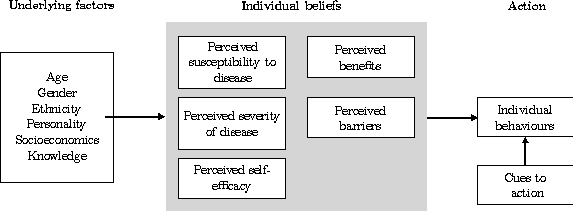
\includegraphics[width=1\textwidth]{figures/ch5/hbm-conceptual-diagram.pdf}
     \end{adjustbox}
    \bcaption{Conceptual formulation of the Health Belief Model.}{Underlying and environmental factors (left) of an individual inform the individual's beliefs (middle) about the disease and available preventive measure(s). Predictions of preventive behaviours (right) are a combination of these beliefs. Adapted from \citet{champion_health_2015}.}
    \label{fig:lit-review-hbm}
\end{figure}

Originally introduced in the 1950s by \citet{hochbaum_public_1958}, and later extended by \citet{becker_health_1974}, the HBM combines factors of individuals to predict whether people will adopt preventive measures for illnesses. There are six components (called \textit{constructs}) of the HBM that combine to predict the likelihood an individual will adopt a preventive measure (shown in Figure~\ref{fig:lit-review-hbm}). These are:

\begin{description}
    \item \textbf{Perceived susceptibility.} Belief regarding the risk or likelihood of contracting the disease.
    \item \textbf{Perceived severity.} Belief about how severe the disease and its consequences are.
    \item \textbf{Perceived benefits.} Belief in the effectiveness of a preventive measure to prevent or alleviate disease.
    \item \textbf{Perceived barriers.} Belief about the potential harm or costs of adopting a preventive measures (e.g., side effects, psychological harms, financial implications, etc.).
    \item \textbf{Cues to action.} Stimuli that trigger the decision-making process of whether to use a preventive measure \cite{janz_health_1984}. These may be internal (e.g., symptoms) or external (e.g., encouragement from social network).
    \item \textbf{Self-efficacy.} Belief about an individual's ability to successfully carry out a preventive measure and produce the expected outcomes \cite{bandura_self-efficacy_1997}.
\end{description}

The HBM is based on the assumption that individuals value avoiding illness, and will practice preventive measures if they expect them to sufficiently prevent or alleviate disease. As \citet{champion_health_2015} describe, the HBM hypothesises that individuals undergo an implicit cost-benefit analysis to weigh the expected benefits of the preventive measure against the perceived barriers before changing their behaviour, only if the perceived threat is sufficiently high\footnote{As \citet{rosenstock_historical_1974} describes, the \q{combined levels of susceptibility and severity provide the energy or force to act and the perception of benefits (minus barriers) provides a preferred path of action.}}.

\begin{figure}[htb!]
     \centering
     \begin{adjustbox}{center}
          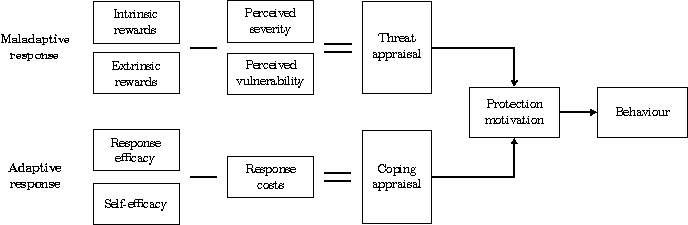
\includegraphics[width=1.2\textwidth]{figures/ch5/pmt-conceptual-diagram.pdf}
     \end{adjustbox}
    \bcaption{Conceptual formulation of Protection Motivation Theory.}{An individual considers the rewards and risk resulting from not adopting the preventive measure (\textit{maladaptive response}) in the threat appraisal. The coping appraisal weighs the benefits and cost of a preventive behaviour (\textit{adaptive response}). These appraisals are compared to predict an individual's resulting behaviour. Adapted from \citet{norman_protection_2015}.}
    \label{fig:lit-review-pmt}
\end{figure}

In a similar vein, PMT was introduced in the 1970s by \citet{rogers_protection_1975} and later refined by the original author \cite{rogers_cognitive_1983}. According to \citet{marikyan_protection_2023}, PMT aimed to address specific psychological and cognitive drivers of protective behaviour that had been previously neglected by other behaviour change theories, such as the HBM. PMT formulates preventive behaviours according to two cognitive appraisals---the theory postulates that individuals assess the significance of a perceived threat (\textit{threat appraisal}) and the available methods of coping with the threat (\textit{coping appraisal}) to determine the behaviour they are most inclined to perform \cite{norman_protection_2015}. The additional constructs included in PMT (shown in Figure~\ref{fig:lit-review-pmt}) are:

\begin{description}
    \item \textbf{Intrinsic rewards.} Inherent rewards of not performing the recommended health behaviour (e.g., pleasure from smoking).
    \item[Extrinsic rewards.] External rewards of not performing the recommended health behaviour (e.g., social approval) \cite{norman_protection_2015}.
    \item \textbf{Response efficacy.} Belief that the preventive measure will effectively protect an individual (or others).
    \item \textbf{Response cost.} Costs associated with adopting a preventive measure (e.g., financial repercussions, time expenditure, effort).
\end{description}

Unlike the HBM, the appraisals in PMT are from the perspective of whether the individual adopts a preventive measure or not. The threat appraisal is the assessment of how severe the disease is without the use of a preventive measure (\textit{maladaptive response}), whereas the coping appraisal weighs the effectiveness of the preventive measure against its costs (\textit{adaptive response}) \cite{leith_motivation_2004}. Each appraisal involves an explicit cost-benefit analysis: The higher the perceived threat and belief in preventive measure efficacy, the higher the likelihood of behaviour change \cite{marikyan_protection_2023}. This explicit comparison of utility in PMT is a major difference that sets it apart from the HBM, despite the two theories sharing many constructs.

While PMT and the HBM have been applied to VBD studies to identify endogenous and exogenous factors that motivate the adoption of preventive measures \cite{vande_velde_integrated_2024, vizanko_modeling_2024, donohoe_tick-borne_2018, ghahremani_effect_2014}, both frameworks have been criticised to varying degrees. For example, \citet{bunton_theories_1991} and others have noted that the HBM fails to \q{incorporate the wider context in which social decision and actions are taken} \cite{williams_role_2010}, and omits the \q{important roles of impulsivity, habit, self-control, associative learning, and emotional progressing} in behaviour change \cite{michie_behaviour_2011}. The HBM also lacks a clear construct for human emotion, despite its suggested importance for behaviour during epidemics \cite{durham_incorporating_2012}. Similarly, PMT has been criticised for lacking a social risk component, despite multiple studies demonstrating the importance of social risk severity perceptions for predicting preventive behaviours in VBD epidemics \cite{lopes-rafegas_contribution_2023, vande_velde_integrated_2024} and other health scenarios \cite{pechmann_what_2003}.

Attempts to address the drawbacks of the HBM and PMT have led to new, comprehensive behaviour change theories, such as the seminal COM-B (Capability, Opportunity, Motivation, and Behaviour) model developed by \citet{michie_behaviour_2011}. Unlike the HBM, COM-B was designed from the ground up to include social and environmental factors that influence behaviour, with a focus on characterising and designing communal interventions. COM-B formulates behaviour change from the perspective of an individual's physical and physiological capability to participate, social and physical opportunity, and sufficient endogenous motivation to adopt a behaviour. Despite these advancements in the fields of psychology and sociology, however, mathematical and computational models that attempt to incorporate such behaviour change theories remain sparse.

\subsubsection{Modelling vector-borne diseases}\label{sec:model-vbds}

From the above discussion, vector control campaigns evidently present a complex challenge: health officials must not only supply effective vector control tools to curb disease transmission, but also consider the intricate socioeconomic factors that influence human behaviour and community participation. Fortunately, mathematical models have emerged as useful tools to guide policy and vector control interventions by modelling the interactions between vector and human populations. The majority of these are compartmental equation-based models (EBMs), typically defined by a system of ordinary differential equations (ODEs) that explicitly represent the population-level dynamics of disease spread.

The SIR (Susceptible, Infected, and Recovered) model is perhaps the most simple and well-known compartmental model in epidemiology, and is defined by the differential equations in Figure~\ref{fig:sir-eqs}, and diagrammatically represented in Figure~\ref{fig:sir-diagram}. In the compartmental SIR model, each compartment ($S$, $I$, or $R$) represents either the number or proportion of individuals in each state. In the latter case shown in Figure~\ref{fig:sir-fig}, the sum of compartments $S+I+R=1$, and the differential equations govern the flow of individuals between states: $\beta$ is the rate of infection, and $1/\gamma$ is the average infectious period.

\begin{figure}[htbp]
     \centering
     \begin{subfigure}[b]{0.3\textwidth}
         \centering
         \begin{align*}
             \dot{S}&=-\beta S I \\
             \dot{I}&=\beta S I - \gamma I \\
             \dot{R}&=\gamma I
         \end{align*}
         \vspace{.5cm}
         \caption{}
         \label{fig:sir-eqs}
     \end{subfigure}%
     \hfill
     \begin{subfigure}[b]{0.3\textwidth}
         \centering
         \begin{tikzpicture}[node distance=1cm, auto,
                >=Latex, 
                every node/.append style={align=center},
                int/.style={draw, thick, minimum width=2cm,minimum height=.6cm,rounded corners}]
            
               \node [int, fill=s-color, text=white] (S)             {$S$};
               \node [int, below=of S, fill=i-color, text=white] (I) {$I$};
               \node [int, below=of I, fill=r-color, text=white] (R) {$R$};
               \coordinate[below=of I] (out);
               \path[->] (S) edge node {$\beta S I$} (I)
                         (I) edge node {$\gamma$} (out);
        \end{tikzpicture}%
        \vspace{.1cm}
         \caption{}
         \label{fig:sir-diagram}
     \end{subfigure}%
     \hfill
     \begin{subfigure}[b]{0.3\textwidth}
         \centering
         \begin{tikzpicture}[x=0.025cm,y=3cm]
      \def\xmax{130.0} % x axis maximum
      \def\ymax{1.025} % y axis maximum
      
      % CURVES
      \draw[very thick,s-color] plot[smooth] coordinates {
        (0.0, 0.998)
        (1.0, 0.9973276981931711)
        (2.0, 0.9964840728072826)
        (3.0, 0.9954259410355902)
        (4.0, 0.9940995088472758)
        (5.0, 0.9924379202498846)
        (6.0, 0.9903583301294537)
        (7.0, 0.9877584623411796)
        (8.0, 0.9845126449693982)
        (9.0, 0.9804673761499587)
        (10.0, 0.9754365737308862)
        (11.0, 0.9691968214949727)
        (12.0, 0.9614831599950985)
        (13.0, 0.9519862997172801)
        (14.0, 0.940352554204059)
        (15.0, 0.9261882782122965)
        (16.0, 0.9090710438495231)
        (17.0, 0.8885700212989189)
        (18.0, 0.8642777263133894)
        (19.0, 0.8358540642118198)
        (20.0, 0.8030810771908262)
        (21.0, 0.7659229280505638)
        (22.0, 0.7245810914666934)
        (23.0, 0.6795310390592031)
        (24.0, 0.6315262208094109)
        (25.0, 0.5815597728549975)
        (26.0, 0.530784287703032)
        (27.0, 0.480401961203948)
        (28.0, 0.4315470131997255)
        (29.0, 0.3851844173656373)
        (30.0, 0.34204311236478063)
        (31.0, 0.30259079319787735)
        (32.0, 0.26704619116159567)
        (33.0, 0.23541747963832935)
        (34.0, 0.20755337693627968)
        (35.0, 0.18319550431436243)
        (36.0, 0.16202449489961224)
        (37.0, 0.14369631108544192)
        (38.0, 0.12786819190459633)
        (39.0, 0.1142154240467327)
        (40.0, 0.10244085770765672)
        (41.0, 0.09227917117513319)
        (42.0, 0.08349762407542727)
        (43.0, 0.07589465262860504)
        (44.0, 0.06929728200938529)
        (45.0, 0.06355801522279642)
        (46.0, 0.058551620655525126)
        (47.0, 0.054172042625136994)
        (48.0, 0.050329592261200325)
        (49.0, 0.04694844269012026)
        (50.0, 0.043964461012344906)
        (51.0, 0.04132334644651637)
        (52.0, 0.038979052841522095)
        (53.0, 0.03689245949626464)
        (54.0, 0.03503025674479982)
        (55.0, 0.0333640148992419)
        (56.0, 0.03186940716069393)
        (57.0, 0.03052556194112793)
        (58.0, 0.029314522922940435)
        (59.0, 0.028220798717186017)
        (60.0, 0.027230986866564763)
        (61.0, 0.02633345947719667)
        (62.0, 0.025518099944165016)
        (63.0, 0.024776082010869227)
        (64.0, 0.024099684200702437)
        (65.0, 0.023482133047441546)
        (66.0, 0.022917471110447615)
        (67.0, 0.02240044496406817)
        (68.0, 0.021926410315262507)
        (69.0, 0.021491251208289104)
        (70.0, 0.02109131113702911)
        (71.0, 0.02072333416281497)
        (72.0, 0.0203844144502876)
        (73.0, 0.020071952916559888)
        (74.0, 0.019783619900088856)
        (75.0, 0.01951732294773462)
        (76.0, 0.019271178924476662)
        (77.0, 0.01904348983513639)
        (78.0, 0.01883272179724266)
        (79.0, 0.018637486725199447)
        (80.0, 0.018456526325907375)
        (81.0, 0.01828869811954071)
        (82.0, 0.01813296312543959)
        (83.0, 0.0179883750995347)
        (84.0, 0.017854070995352137)
        (85.0, 0.017729262582964676)
        (86.0, 0.017613229006327027)
        (87.0, 0.017505310212865357)
        (88.0, 0.017404901096874745)
        (89.0, 0.0173114462974976)
        (90.0, 0.017224435562151353)
        (91.0, 0.017143399595539257)
        (92.0, 0.01706790635057259)
        (93.0, 0.016997557715887304)
        (94.0, 0.016931986521943748)
        (95.0, 0.016870853839826203)
        (96.0, 0.016813846588184817)
        (97.0, 0.016760675318771994)
        (98.0, 0.016711072272525326)
        (99.0, 0.016664789559655245)
        (100.0, 0.016621597566351946)
        (101.0, 0.01658128346014513)
        (102.0, 0.01654364986963487)
        (103.0, 0.016508513649971912)
        (104.0, 0.01647570478322638)
        (105.0, 0.016445065355601956)
        (106.0, 0.016416448635980945)
        (107.0, 0.01638971822340957)
        (108.0, 0.01636474727181619)
        (109.0, 0.016341417776474017)
        (110.0, 0.01631961991911177)
        (111.0, 0.016299251466096593)
        (112.0, 0.01628021721595586)
        (113.0, 0.016262428496385112)
        (114.0, 0.01624580267822401)
        (115.0, 0.016230262760800425)
        (116.0, 0.016215736962871975)
        (117.0, 0.01620215835153872)
        (118.0, 0.016189464506740366)
        (119.0, 0.016177597205375163)
        (120.0, 0.016166502123166716)
        (121.0, 0.01615612857185693)
        (122.0, 0.01614642924562425)
        (123.0, 0.016137359984575585)
        (124.0, 0.016128879567973667)
        (125.0, 0.01612094950436089)
      } node[above right] at (20.0, 0.85) {$S$};
    
      \draw[very thick,i-color] plot[smooth] coordinates {
        (0.0, 0.002)
        (1.0, 0.0025118551142537743)
        (2.0, 0.0031539938777885444)
        (3.0, 0.0039591662695688465)
        (4.0, 0.004968118489808619)
        (5.0, 0.00623140960500875)
        (6.0, 0.007811562939418319)
        (7.0, 0.009785566255793595)
        (8.0, 0.012247703979930483)
        (9.0, 0.015312646690744908)
        (10.0, 0.019118631546431588)
        (11.0, 0.023830424406796634)
        (12.0, 0.029641548066158235)
        (13.0, 0.036774978103104934)
        (14.0, 0.04548115670733093)
        (15.0, 0.056031784071024576)
        (16.0, 0.06870752067429403)
        (17.0, 0.08377764007513508)
        (18.0, 0.10147010366212483)
        (19.0, 0.12193183146840725)
        (20.0, 0.14518140067848814)
        (21.0, 0.17105999575147074)
        (22.0, 0.19919043532171044)
        (23.0, 0.22895696958160838)
        (24.0, 0.259518106856763)
        (25.0, 0.28985938667094235)
        (26.0, 0.3188829532686558)
        (27.0, 0.3455194399114178)
        (28.0, 0.3688394565809396)
        (29.0, 0.3881415222032409)
        (30.0, 0.4030005812795563)
        (31.0, 0.4132730399035242)
        (32.0, 0.41906532352012577)
        (33.0, 0.42067946344958507)
        (34.0, 0.4185502560260349)
        (35.0, 0.41318559720843967)
        (36.0, 0.40511699252513234)
        (37.0, 0.39486293867085376)
        (38.0, 0.3829048359712472)
        (39.0, 0.3696734068745041)
        (40.0, 0.35554304142539545)
        (41.0, 0.34083158946059094)
        (42.0, 0.32580354734024025)
        (43.0, 0.31067510055440883)
        (44.0, 0.29561995717048395)
        (45.0, 0.28077527980532796)
        (46.0, 0.26624730330554247)
        (47.0, 0.25211645104600255)
        (48.0, 0.2384418197612011)
        (49.0, 0.22526506832660712)
        (50.0, 0.21261370867495347)
        (51.0, 0.20050387694464075)
        (52.0, 0.1889426384526646)
        (53.0, 0.17792989454199318)
        (54.0, 0.16745995095769076)
        (55.0, 0.1575228009041371)
        (56.0, 0.1481051718320928)
        (57.0, 0.13919137482870902)
        (58.0, 0.13076399175912412)
        (59.0, 0.12280442866621256)
        (60.0, 0.11529335930002195)
        (61.0, 0.10821107868483248)
        (62.0, 0.10153778306609723)
        (63.0, 0.09525378974173093)
        (64.0, 0.08933970751617225)
        (65.0, 0.08377656795680846)
        (66.0, 0.07854592336352069)
        (67.0, 0.07362991889742818)
        (68.0, 0.06901134319755721)
        (69.0, 0.06467366191877792)
        (70.0, 0.06060103750187934)
        (71.0, 0.056778337871093404)
        (72.0, 0.053191136511508266)
        (73.0, 0.04982570562316056)
        (74.0, 0.04666900390809084)
        (75.0, 0.04370866035237411)
        (76.0, 0.04093295490047132)
        (77.0, 0.03833079688115406)
        (78.0, 0.03589170191195289)
        (79.0, 0.033605767757493035)
        (80.0, 0.0314636496459622)
        (81.0, 0.029456535300379883)
        (82.0, 0.02757612011540257)
        (83.0, 0.025814582538337398)
        (84.0, 0.024164559970481298)
        (85.0, 0.022619125203910007)
        (86.0, 0.021171763595026684)
        (87.0, 0.01981635095076292)
        (88.0, 0.018547132265826043)
        (89.0, 0.017358701287442397)
        (90.0, 0.016245980943696357)
        (91.0, 0.015204204657283225)
        (92.0, 0.014228898518535435)
        (93.0, 0.013315864297351382)
        (94.0, 0.012461163329890494)
        (95.0, 0.011661101240363472)
        (96.0, 0.010912213393931912)
        (97.0, 0.0102112512067788)
        (98.0, 0.0095551691146386)
        (99.0, 0.008941112345388831)
        (100.0, 0.008366405291875594)
        (101.0, 0.007828540611958488)
        (102.0, 0.007325168898255837)
        (103.0, 0.00685408898038212)
        (104.0, 0.00641323876526587)
        (105.0, 0.00600068664013983)
        (106.0, 0.005614623366158602)
        (107.0, 0.00525335446207554)
        (108.0, 0.004915293041732614)
        (109.0, 0.004598953085528574)
        (110.0, 0.004302943118755094)
        (111.0, 0.004025960273615112)
        (112.0, 0.003766784714830889)
        (113.0, 0.003524274404150664)
        (114.0, 0.003297360197385097)
        (115.0, 0.00308504122679214)
        (116.0, 0.0028863805892277226)
        (117.0, 0.0027005012887202306)
        (118.0, 0.002526582425212876)
        (119.0, 0.0023638556598361343)
        (120.0, 0.002211601837857245)
        (121.0, 0.0020691478868978476)
        (122.0, 0.0019358638729487004)
        (123.0, 0.001811160237143461)
        (124.0, 0.0016944852515148568)
        (125.0, 0.0015853225676223741)
        } node[above right] at (45.0, 0.3) {$I$};
    
        \draw[very thick,r-color] plot[smooth] coordinates {
        (0.0, 0.0)
        (1.0, 0.00016044669257483907)
        (2.0, 0.00036193331492854905)
        (3.0, 0.0006148926948404921)
        (4.0, 0.0009323726629151103)
        (5.0, 0.001330670145106066)
        (6.0, 0.001830106931127467)
        (7.0, 0.002455971403026405)
        (8.0, 0.0032396510506710074)
        (9.0, 0.004219977159296082)
        (10.0, 0.005444794722681841)
        (11.0, 0.006972754098230427)
        (12.0, 0.00887529193874307)
        (13.0, 0.011238722179614701)
        (14.0, 0.014166289088609818)
        (15.0, 0.017779937716678768)
        (16.0, 0.022221435476182713)
        (17.0, 0.027652338625945735)
        (18.0, 0.034252170024485565)
        (19.0, 0.0422141043197727)
        (20.0, 0.05173752213068529)
        (21.0, 0.06301707619796504)
        (22.0, 0.07622847321159593)
        (23.0, 0.09151199135918818)
        (24.0, 0.10895567233382564)
        (25.0, 0.12858084047405985)
        (26.0, 0.1503327590283119)
        (27.0, 0.17407859888463387)
        (28.0, 0.1996135302193346)
        (29.0, 0.22667406043112157)
        (30.0, 0.2549563063556628)
        (31.0, 0.2841361668985982)
        (32.0, 0.31388848531827834)
        (33.0, 0.34390305691208545)
        (34.0, 0.3738963670376853)
        (35.0, 0.40361889847719784)
        (36.0, 0.4328585125752554)
        (37.0, 0.46144075024370435)
        (38.0, 0.48922697212415656)
        (39.0, 0.5161111690787633)
        (40.0, 0.542016100866948)
        (41.0, 0.566889239364276)
        (42.0, 0.5906988285843326)
        (43.0, 0.6134302468169863)
        (44.0, 0.635082760820131)
        (45.0, 0.6556667049718758)
        (46.0, 0.6752010760389326)
        (47.0, 0.6937115063288607)
        (48.0, 0.7112285879775989)
        (49.0, 0.7277864889832728)
        (50.0, 0.7434218303127018)
        (51.0, 0.7581727766088432)
        (52.0, 0.7720783087058135)
        (53.0, 0.7851776459617423)
        (54.0, 0.7975097922975096)
        (55.0, 0.8091131841966213)
        (56.0, 0.8200254210072134)
        (57.0, 0.8302830632301633)
        (58.0, 0.8399214853179355)
        (59.0, 0.8489747726166015)
        (60.0, 0.8574756538334134)
        (61.0, 0.865455461837971)
        (62.0, 0.8729441169897378)
        (63.0, 0.8799701282473998)
        (64.0, 0.8865606082831254)
        (65.0, 0.89274129899575)
        (66.0, 0.8985366055260318)
        (67.0, 0.9039696361385037)
        (68.0, 0.9090622464871803)
        (69.0, 0.913835086872933)
        (70.0, 0.9183076513610916)
        (71.0, 0.9224983279660917)
        (72.0, 0.9264244490382042)
        (73.0, 0.9301023414602796)
        (74.0, 0.9335473761918203)
        (75.0, 0.9367740166998912)
        (76.0, 0.939795866175052)
        (77.0, 0.9426257132837095)
        (78.0, 0.9452755762908044)
        (79.0, 0.9477567455173074)
        (80.0, 0.9500798240281304)
        (81.0, 0.9522547665800793)
        (82.0, 0.9542909167591578)
        (83.0, 0.9561970423621279)
        (84.0, 0.9579813690341665)
        (85.0, 0.9596516122131252)
        (86.0, 0.9612150073986462)
        (87.0, 0.9626783388363717)
        (88.0, 0.9640479666372991)
        (89.0, 0.9653298524150598)
        (90.0, 0.9665295834941521)
        (91.0, 0.9676523957471773)
        (92.0, 0.9687031951308919)
        (93.0, 0.9696865779867614)
        (94.0, 0.9706068501481657)
        (95.0, 0.9714680449198103)
        (96.0, 0.9722739400178834)
        (97.0, 0.9730280734744492)
        (98.0, 0.9737337586128361)
        (99.0, 0.9743940980949559)
        (100.0, 0.9750119971417724)
        (101.0, 0.9755901759278963)
        (102.0, 0.9761311812321092)
        (103.0, 0.9766373973696458)
        (104.0, 0.9771110564515075)
        (105.0, 0.977554248004258)
        (106.0, 0.9779689279978604)
        (107.0, 0.9783569273145148)
        (108.0, 0.9787199596864512)
        (109.0, 0.9790596291379974)
        (110.0, 0.9793774369621331)
        (111.0, 0.9796747882602882)
        (112.0, 0.9799529980692132)
        (113.0, 0.9802132970994641)
        (114.0, 0.9804568371243909)
        (115.0, 0.9806846960124074)
        (116.0, 0.9808978824479002)
        (117.0, 0.9810973403597408)
        (118.0, 0.9812839530680466)
        (119.0, 0.9814585471347885)
        (120.0, 0.981621896038976)
        (121.0, 0.9817747235412451)
        (122.0, 0.9819177068814269)
        (123.0, 0.9820514797782809)
        (124.0, 0.9821766351805113)
        (125.0, 0.9822937279280166)
        } node[above right] at (75.0, 0.775) {$R$};

        % AXES
      \draw[<->,thick]
        (\xmax,0) node[below left] {$t$}
        -| (0,\ymax) node[above left,rotate=90] {Proportion};
    \end{tikzpicture}%
    \vspace{.05cm}
         \caption{}
         \label{fig:sir-curve}
     \end{subfigure}%
        \bcaption{Compartmental SIR model.}{\textbf{(i)} System of differential equations representing changes in flows between compartments. \textbf{(ii)} Compartmental diagram representing flows between compartments. \textbf{(iii)} SIR dynamics over time for $\beta=0.3$ and $1/\gamma=14$.}
        \label{fig:sir-fig}
\end{figure}

Compartmental models that extend the SIR model have long been used in epidemiological and VBD contexts \cite{tang_review_2020}. In his review, \citet{cosner_models_2015} covered spatial and non-spatial EBMs for VBDs, noting that \q{even simple models can provide insights into how movement patterns can affect disease transmission.} More complex EBMs have incorporated vector control tools such as medicine and insecticide spraying to analyse the efficacy and timeliness of these interventions \cite{reiner_systematic_2013}. Despite the success of these models, however, they are limited in that populations are assumed to be homogeneous, meaning infection rates and other factors such as mosquito biting rates are constant, despite studies suggesting otherwise \cite{perkins_heterogeneity_2013}. During their review of almost 400 equation-based VBD models from 1970 to 2010, \citet{reiner_systematic_2013} noted that most modern VBD models still employ \q{basic transmission dynamics} closely resembling the original Ross-Macdonald malaria model \cite{ross_report_1908,macdonald_epidemiology_1957}, and claimed the field could benefit from models that incorporate heterogeneity.

Despite the assumption of homogeneous populations in EBMs, recent research has investigated methods of facilitating heterogeneity in these models. For example, \citet{perkins_heterogeneity_2013} proposed a framework for heterogeneous mosquito biting rates, transmission thresholds, and spatial scales of transmission by defining sub-populations of mosquitoes characterised by different systems of equations. These \textit{patch} (or \textit{metapopulation}) models are a common technique used to create discrete heterogeneous groups within EBMs: \citet{suarez_generic_2020} used the technique to incorporate varied risk perception and demand for vector control. Similarly, \citet{roosa_general_2022} combined a patch model with an extended compartmental SIR model to study uptake dynamics of preventive measures.

Alternative mathematical techniques such as artificial intelligence or machine learning have also been applied in VBD contexts. These methods aim to identify relationships from data without defining underlying representations of transmission mechanisms, and are mainly used to predict and forecast future VBD risk scenarios \cite{judson_modeling_2024}. For example, \citet{peters_big_2020} used machine learning with big data sources to predict the expansion of a VBD in the Americas. Similarly, \citet{pandit_predicting_2022} used statistical data-driven network modelling techniques to predict the transmission of various zoonotic diseases. While such techniques may be useful for forecasting purposes, predictive transmission models may not be as effective in guiding policy or informing health officials' understanding of disease spread patterns due to the \q{black box} nature such approaches. Furthermore, artificial intelligence techniques often require large amounts of data to be effective, which can be particularly prohibitive in VBD contexts due to underdeveloped surveillance infrastructure in affected countries \cite{okumu_what_2022}.

Overall, both EBMs and statistical machine learning methods are arguably not well suited for investigating the dynamics between preventive behaviours and VBD spread. In the case of EBMs, the well-mixed assumption implies that individual behavioural attitudes are invariant over time within populations \cite{bedson_review_2021}. Statistical and machine learning approaches, on the other hand, have no dimension for modelling behavioural processes due to their non-mechanistic nature. Instead, these techniques can only attempt to infer linkages between infection risk and preventive behaviours, such as in \citet{aerts_understanding_2020}. In sum, this general lack of consideration for behaviour and individual-level interactions in such models disregards the important contextual underpinnings that drive heterogeneous preventive behaviours within communities \cite{bedson_review_2021}.

\subsection{Agent-based modelling}\label{lr-abm}

The inability of EBMs to incorporate heterogeneity and the drawbacks of pure statistical methods outlined above are reasons why modellers may turn to agent-based models (ABMs) for modelling VBDs. Contrary to the top-down specification EBMs require, ABMs define a population of decentralised, autonomous agents that interact with one another to reproduce or \q{grow} emergent phenomena \cite{epstein_growing_1996}. Unlike the fixed system structure of EBMs, ABMs typically consist of simple rules that can be readily changed to alter system mechanisms. This \textit{bottom-up} approach naturally incorporates heterogeneity and the adaptation of agents \cite{axtell_agent-based_2022}, greatly simplifying representations of interventions or hypothetical scenarios \cite{van_dyke_parunak_agent-based_1998}. In the context of epidemiology, an ABM can thus \q{function as an \textit{in silico} laboratory} for health practitioners to simulate populations with heterogeneous biological, spatial, and behavioural characteristics \cite{marshall_formalizing_2015}.

\begin{figure}[h]
\centering

\begin{tikzpicture}[scale=1.1]
    \def\ioffset{0.525} % x axis maximum
    \def\matsize{5}
    
    % Draw labels
    \foreach \i in {0,1}
        \path (\i+\ioffset,-1+\ioffset) node{\i} (-1+\ioffset,\i+\ioffset) node{\i};
    \path (2+\ioffset,-1+\ioffset) node{$\dots$} (-1+\ioffset,2+\ioffset) node[rotate=90] {$\dots$};
    \path (3+\ioffset,-1+\ioffset) node{$i$} (-1+\ioffset,3+\ioffset) node{$j$};
    \path (4+\ioffset,-1+\ioffset) node{$\dots$} (-1+\ioffset,4+\ioffset) node[rotate=90] {$\dots$};
    \path (\matsize+\ioffset,-1+\ioffset) node{$N_b$} (-1+\ioffset,\matsize+\ioffset) node{$N_b$};
      
    % Draw lattice rects
    \foreach \i in {0,...,\matsize}
        \foreach \j in {0,...,\matsize}{
            % Check if current cell is (1,2) or (3,4) and color green
            \ifthenelse{\(\i=0 \AND \j=0\) \OR \(\i=0 \AND \j=2\) \OR \(\i=0 \AND \j=3\) \OR \(\i=0 \AND \j=4\) \OR \(\i=1 \AND \j=0\) \OR \(\i=1 \AND \j=1\) \OR \(\i=1 \AND \j=2\) \OR \(\i=2 \AND \j=0\) \OR \(\i=2 \AND \j=1\) \OR \(\i=2 \AND \j=2\) \OR \(\i=2 \AND \j=4\) \OR \(\i=3 \AND \j=1\) \OR \(\i=3 \AND \j=3\) \OR \(\i=3 \AND \j=4\) \OR \(\i=4 \AND \j=0\) \OR \(\i=4 \AND \j=4\) \OR \(\i=4 \AND \j=5\) \OR \(\i=5 \AND \j=0\) \OR \(\i=5 \AND \j=3\) \OR \(\i=5 \AND \j=4\)}{
                \fill[s-color] (\i+0.1,\j+0.1) rectangle (\i+0.95,\j+0.95);
            }{}

            \ifthenelse{\(\i=3 \AND \j=0\) \OR \(\i=4 \AND \j=3\) \OR \(\i=4 \AND \j=2\) \OR \(\i=2 \AND \j=5\)}{
                \fill[i-color] (\i+0.1,\j+0.1) rectangle (\i+0.95,\j+0.95);
            }{}

            \ifthenelse{\(\i=1 \AND \j=5\) \OR \(\i=5 \AND \j=5\) \OR \(\i=4 \AND \j=1\)}{
                \fill[r-color] (\i+0.1,\j+0.1) rectangle (\i+0.95,\j+0.95);
            }{}

            
            \draw[thick] (\i+0.1,\j+0.1) rectangle (\i+0.95,\j+0.95);
        };

    % Draw agents
    % R agents
    % \node[person,shirt=r-color,scale=1.2] at (1.1+\ioffset,5.3+\ioffset) {};
    % \node[person,shirt=r-color,scale=1.2] at (1-.1+\ioffset,5+\ioffset) {};
    
    % S agents
    % \node[person,shirt=s-color,scale=1.2] at (1-.1+\ioffset,1-.1+\ioffset) {};
    
    % \node[person,shirt=s-color,scale=1.2] at (2.1+\ioffset,1.3+\ioffset) {};
    % \node[person,shirt=s-color,scale=1.2] at (2-.1+\ioffset,1+\ioffset) {};

    % I agents
    % \node[black,scale=1.1] at (3-.1+\ioffset,0.1+\ioffset) {\usymH{1F6B9}{.9cm}};
    % \node[i-color] at (3-.1+\ioffset,0.1+\ioffset) {\usymH{1F6B9}{.8cm}};
    % \node[i-color] at (3-.1+\ioffset,0.1+\ioffset) {};

    \node[isosceles triangle, isosceles triangle apex angle=90, fill=s-color, minimum size=.66cm, rotate=225] at (4.38,2.37) {};
    \draw[thick] (4+0.1,2+0.1) rectangle (4+0.95,2+0.95);

    \newcommand{\drawagent}[1]{
    \path[draw=black,fill=#1,miter limit=10.0,scale=.3] (1.6431, -0.2275).. controls (1.5055, -0.2275) and (1.3944, -0.3387) .. (1.3944, -0.4763).. controls (1.3944, -0.6138) and (1.5055, -0.725) .. (1.6431, -0.725).. controls (1.7806, -0.725) and (1.8918, -0.6138) .. (1.8918, -0.4763).. controls (1.8918, -0.3387) and (1.7806, -0.2275) .. (1.6431, -0.2275) -- cycle(1.3679, -0.7911).. controls (1.1906, -0.7911) and (1.0478, -0.934) .. (1.0478, -1.1113) -- (1.0478, -1.8838).. controls (1.0478, -1.9447) and (1.0954, -1.9923) .. (1.1562, -1.9923).. controls (1.2171, -1.9923) and (1.2647, -1.9447) .. (1.2647, -1.8838) -- (1.2647, -1.1853) -- (1.3203, -1.1853).. controls (1.3203, -1.1853) and (1.3203, -3.0057) .. (1.3203, -3.1247).. controls (1.3203, -3.2041) and (1.3864, -3.2703) .. (1.4658, -3.2703).. controls (1.5478, -3.2703) and (1.6113, -3.2041) .. (1.6113, -3.1247) -- (1.6113, -1.9976) -- (1.6722, -1.9976) -- (1.6722, -3.1247).. controls (1.6722, -3.2041) and (1.7383, -3.2703) .. (1.8177, -3.2703).. controls (1.8997, -3.2703) and (1.9632, -3.2041) .. (1.9632, -3.1247) -- (1.9632, -1.1853) -- (2.0188, -1.1853) -- (2.0188, -1.8838).. controls (2.0188, -1.9447) and (2.0664, -1.9923) .. (2.1273, -1.9923).. controls (2.1881, -1.9923) and (2.2357, -1.9447) .. (2.2357, -1.8838) -- (2.2357, -1.1086).. controls (2.2357, -0.9313) and (2.0902, -0.7885) .. (1.9156, -0.7885).. controls (1.9182, -0.7911) and (1.3679, -0.7911) .. (1.3679, -0.7911) -- cycle;
    }

    \newcommand{\drawagentat}[3]{
    \tikzset{shift={(#2,#3)}}
    
    \path[draw=black,fill=#1,miter limit=10.0,scale=.3] (1.6431, -0.2275).. controls (1.5055, -0.2275) and (1.3944, -0.3387) .. (1.3944, -0.4763).. controls (1.3944, -0.6138) and (1.5055, -0.725) .. (1.6431, -0.725).. controls (1.7806, -0.725) and (1.8918, -0.6138) .. (1.8918, -0.4763).. controls (1.8918, -0.3387) and (1.7806, -0.2275) .. (1.6431, -0.2275) -- cycle(1.3679, -0.7911).. controls (1.1906, -0.7911) and (1.0478, -0.934) .. (1.0478, -1.1113) -- (1.0478, -1.8838).. controls (1.0478, -1.9447) and (1.0954, -1.9923) .. (1.1562, -1.9923).. controls (1.2171, -1.9923) and (1.2647, -1.9447) .. (1.2647, -1.8838) -- (1.2647, -1.1853) -- (1.3203, -1.1853).. controls (1.3203, -1.1853) and (1.3203, -3.0057) .. (1.3203, -3.1247).. controls (1.3203, -3.2041) and (1.3864, -3.2703) .. (1.4658, -3.2703).. controls (1.5478, -3.2703) and (1.6113, -3.2041) .. (1.6113, -3.1247) -- (1.6113, -1.9976) -- (1.6722, -1.9976) -- (1.6722, -3.1247).. controls (1.6722, -3.2041) and (1.7383, -3.2703) .. (1.8177, -3.2703).. controls (1.8997, -3.2703) and (1.9632, -3.2041) .. (1.9632, -3.1247) -- (1.9632, -1.1853) -- (2.0188, -1.1853) -- (2.0188, -1.8838).. controls (2.0188, -1.9447) and (2.0664, -1.9923) .. (2.1273, -1.9923).. controls (2.1881, -1.9923) and (2.2357, -1.9447) .. (2.2357, -1.8838) -- (2.2357, -1.1086).. controls (2.2357, -0.9313) and (2.0902, -0.7885) .. (1.9156, -0.7885).. controls (1.9182, -0.7911) and (1.3679, -0.7911) .. (1.3679, -0.7911) -- cycle;

    \tikzset{shift={(-#2,-#3)}}
    }

    % S agents
    \tikzset{shift={(.4+\ioffset,1.7+\ioffset)}}
        \drawagent{s-color}
    \tikzset{shift={(1.25,.25)}}
        \drawagent{s-color}
    \tikzset{shift={(-.35,-.25)}}
        \drawagent{s-color}

    % R agents
    \tikzset{shift={(-.95,4.2)}}
        \drawagent{r-color}
    \tikzset{shift={(.3,-.1)}}
        \drawagent{r-color}
    \tikzset{shift={(-.2,-.15)}}
        \drawagent{r-color}

    % I agent
    \tikzset{shift={(1.85,-4.7)}}
        \drawagent{i-color}

    % S and I agent
    \tikzset{shift={(1.4,2.05)}}
        \drawagent{i-color}
    \tikzset{shift={(-.35,-.23)}}
        \drawagent{s-color}

    % Equations
    \tikzset{shift={(3.25, 1.8)}}
    \node[] at (0,0) {\textbf{(a)}};
    \drawagentat{s-color}{0.2}{-.1}
    \drawagentat{i-color}{0.6}{-.8}
    \path[->, draw, thick] (1.8, -1) -- (3, -1);
    \node at (2.4, -.7) {$\beta$};
    
    \drawagentat{i-color}{3.1}{-.1}
    \drawagentat{i-color}{3.5}{-.8}

    \tikzset{shift={(0, -3)}}
    \node[] at (0,0) {\textbf{(b)}};
    \drawagentat{i-color}{0.4}{-.1}
    \path[->, draw, thick] (1.6, -.5) -- (3, -.5);
    \node at (2.2, -.2) {$\gamma$};
    \drawagentat{r-color}{3.1}{-.1}
    
    
\end{tikzpicture}

\bcaption{Example ABM of SIR dynamics on a lattice.}{Agents with different SIR states move randomly from any cell to any orthogonally adjacent cell. Teal agents are susceptible, red agents are infected, and purple agents are recovered. Not all agents are shown. (Multi-)coloured cells correspond to the SIR state of agents within that cell, and white cells are unoccupied. \textbf{(a)} Susceptible agents that share a cell with infected agents are infected with probability $\beta$ during each time step. \textbf{(b)} Infected agents recover after an average $1/\gamma$ time steps. Adapted from \citet{paoluzzi_single-agent_2021}.}
\label{sir-abm-diag}
\end{figure}

A corollary of the malleable structure of ABMs is that existing models can be easily extended for different purposes. One example is the discrete agent-based representation of the SIR model illustrated in Figure~\ref{sir-abm-diag} where $N$ agents move randomly about an $N_b\times N_b$ lattice. If an infected agent and a susceptible agent occupy the same cell at any given time step, the susceptible agent is infected with probability $\beta$. Similar to the equation-based form, after an average $1/\gamma$ time steps, infected agents recover from the disease. The simple ABM SIR model has been extended by, for example, \citet{paoluzzi_single-agent_2021}, who alter agent mobility to investigate the impacts of restrictions during the COVID-19 epidemic. Notably in this example, stochasticity is incorporated through the random movement of agents---unlike EBMs, this addition of stochasticity means simulations must be repeated and their results aggregated to draw conclusions about model dynamics.

% \begin{figure}[htbp]
    \centering

    \begin{tikzpicture}[>=stealth]
    % LHS plot 1
    \draw[curve,s-color] plot[smooth] coordinates {
    (-8.0, 3.49)
    (-7.724024512482009, 3.3899999999999997)
    (-7.6484637396372115, 3.3200000000000003)
    (-7.575293451467849, 3.26)
    (-7.503363558513278, 3.17)
    (-7.431975571153575, 3.1)
    (-7.4034740477674585, 3.04)
    (-7.347587243310602, 2.9699999999999998)
    (-7.319165044453064, 2.92)
    (-7.295761688316618, 2.85)
    (-7.256915998988681, 2.79)
    (-7.227168918566119, 2.73)
    (-7.214826797701855, 2.6399999999999997)
    (-7.190112056349427, 2.56)
    (-7.145799388697578, 2.51)
    (-7.114025393756335, 2.43)
    (-7.083940841055886, 2.4)
    (-7.065913148865518, 2.34)
    (-7.040632834972005, 2.2800000000000002)
    (-7.020523178328933, 2.21)
    (-6.994840986408573, 2.13)
    (-6.964917234604183, 2.07)
    (-6.935920958726876, 2.01)
    (-6.90240456136456, 1.96)
    (-6.871291715913282, 1.92)
    (-6.8479224101567615, 1.87)
    (-6.818213573307265, 1.83)
    (-6.776110138898, 1.78)
    (-6.700132590103333, 1.75)
    (-6.658815900705981, 1.74)
    (-6.57460720665217, 1.7)
    (-6.529765752224526, 1.68)
    (-6.45546739165365, 1.67)
    (-6.410288267674974, 1.65)
    (-6.332084009436284, 1.62)
    (-6.292160628893704, 1.59)
    (-6.164451622325407, 1.57)
    (-5.948722216423396, 1.57)
    (-5.5, 1.57)
    };
    
    \draw[curve,i-color] plot[smooth] coordinates {
    (-8.0, 1.51)
    (-7.724024512482009, 1.61)
    (-7.6484637396372115, 1.65)
    (-7.575293451467849, 1.67)
    (-7.503363558513278, 1.75)
    (-7.431975571153575, 1.79)
    (-7.4034740477674585, 1.81)
    (-7.347587243310602, 1.85)
    (-7.319165044453064, 1.85)
    (-7.295761688316618, 1.8900000000000001)
    (-7.256915998988681, 1.91)
    (-7.227168918566119, 1.93)
    (-7.214826797701855, 2.01)
    (-7.190112056349427, 2.07)
    (-7.145799388697578, 2.07)
    (-7.114025393756335, 2.13)
    (-7.083940841055886, 2.09)
    (-7.065913148865518, 2.11)
    (-7.040632834972005, 2.13)
    (-7.020523178328933, 2.17)
    (-6.994840986408573, 2.23)
    (-6.964917234604183, 2.25)
    (-6.935920958726876, 2.27)
    (-6.90240456136456, 2.27)
    (-6.871291715913282, 2.25)
    (-6.8479224101567615, 2.25)
    (-6.818213573307265, 2.23)
    (-6.776110138898, 2.23)
    (-6.700132590103333, 2.19)
    (-6.658815900705981, 2.11)
    (-6.57460720665217, 2.09)
    (-6.529765752224526, 2.0300000000000002)
    (-6.45546739165365, 1.95)
    (-6.410288267674974, 1.8900000000000001)
    (-6.332084009436284, 1.85)
    (-6.292160628893704, 1.81)
    (-6.164451622325407, 1.75)
    (-5.948722216423396, 1.65)
    (-5.5, 1.55)
    };
    
    \draw[curve,r-color] plot[smooth] coordinates {
    (-8.0, 1.5)
    (-7.724024512482009, 1.5)
    (-7.6484637396372115, 1.53)
    (-7.575293451467849, 1.57)
    (-7.503363558513278, 1.58)
    (-7.431975571153575, 1.61)
    (-7.4034740477674585, 1.65)
    (-7.347587243310602, 1.68)
    (-7.319165044453064, 1.73)
    (-7.295761688316618, 1.76)
    (-7.256915998988681, 1.8)
    (-7.227168918566119, 1.84)
    (-7.214826797701855, 1.85)
    (-7.190112056349427, 1.87)
    (-7.145799388697578, 1.92)
    (-7.114025393756335, 1.94)
    (-7.083940841055886, 2.01)
    (-7.065913148865518, 2.05)
    (-7.040632834972005, 2.09)
    (-7.020523178328933, 2.12)
    (-6.994840986408573, 2.14)
    (-6.964917234604183, 2.18)
    (-6.935920958726876, 2.2199999999999998)
    (-6.90240456136456, 2.27)
    (-6.871291715913282, 2.33)
    (-6.8479224101567615, 2.38)
    (-6.818213573307265, 2.44)
    (-6.776110138898, 2.49)
    (-6.700132590103333, 2.56)
    (-6.658815900705981, 2.65)
    (-6.57460720665217, 2.71)
    (-6.529765752224526, 2.79)
    (-6.45546739165365, 2.88)
    (-6.410288267674974, 2.96)
    (-6.332084009436284, 3.0300000000000002)
    (-6.292160628893704, 3.1)
    (-6.164451622325407, 3.1799999999999997)
    (-5.948722216423396, 3.2800000000000002)
    (-5.5, 3.38)
    };
    \draw[->,thick] (-8, 1.5) -- (-5.5, 1.5) node[below left] {$t$};
    \draw[->,thick] (-8, 1.5) -- (-8, 3.5) node[left] {$N$};

    % Dots sep
    \node[rotate=90] at (-7, 0.5) {$\dots$};

    % LHS plot 2
    \draw[curve,s-color] plot[smooth] coordinates {
    (-8.0, -0.010000000000000009)
    (-7.675905625901207, -0.10000000000000009)
    (-7.621177873639785, -0.1399999999999999)
    (-7.489215140697653, -0.17999999999999994)
    (-7.313191941569358, -0.26)
    (-7.265868612764226, -0.3500000000000001)
    (-7.2125195166257425, -0.41999999999999993)
    (-7.178492874106199, -0.47)
    (-7.1128509571699565, -0.54)
    (-7.056309963409815, -0.6100000000000001)
    (-7.026302877482503, -0.6799999999999999)
    (-7.007564697872866, -0.74)
    (-6.98289200110431, -0.81)
    (-6.9625713352402165, -0.8899999999999999)
    (-6.942163035482007, -0.97)
    (-6.9188938759677345, -1.01)
    (-6.90205091717434, -1.08)
    (-6.882410313609648, -1.13)
    (-6.82859443430481, -1.19)
    (-6.808009913481963, -1.25)
    (-6.789774262276251, -1.3199999999999998)
    (-6.7655252416613365, -1.3900000000000001)
    (-6.749582998055055, -1.4300000000000002)
    (-6.694128785342196, -1.48)
    (-6.656313058529874, -1.51)
    (-6.636879919955421, -1.52)
    (-6.597415012880587, -1.56)
    (-6.576119689438654, -1.58)
    (-6.536477553994184, -1.6099999999999999)
    (-6.492760121430862, -1.67)
    (-6.441313105638984, -1.68)
    (-6.381648323533211, -1.69)
    (-6.28967941046716, -1.69)
    (-6.160565722289649, -1.72)
    (-5.901152655592379, -1.75)
    (-5.5, -1.77)
    };
    
    \draw[curve,i-color] plot[smooth] coordinates {
    (-8.0, -1.99)
    (-7.675905625901207, -1.91)
    (-7.621177873639785, -1.93)
    (-7.489215140697653, -1.95)
    (-7.313191941569358, -1.89)
    (-7.265868612764226, -1.81)
    (-7.2125195166257425, -1.77)
    (-7.178492874106199, -1.77)
    (-7.1128509571699565, -1.73)
    (-7.056309963409815, -1.69)
    (-7.026302877482503, -1.65)
    (-7.007564697872866, -1.63)
    (-6.98289200110431, -1.59)
    (-6.9625713352402165, -1.53)
    (-6.942163035482007, -1.47)
    (-6.9188938759677345, -1.49)
    (-6.90205091717434, -1.45)
    (-6.882410313609648, -1.45)
    (-6.82859443430481, -1.4300000000000002)
    (-6.808009913481963, -1.4100000000000001)
    (-6.789774262276251, -1.37)
    (-6.7655252416613365, -1.33)
    (-6.749582998055055, -1.35)
    (-6.694128785342196, -1.35)
    (-6.656313058529874, -1.3900000000000001)
    (-6.636879919955421, -1.47)
    (-6.597415012880587, -1.49)
    (-6.576119689438654, -1.55)
    (-6.536477553994184, -1.59)
    (-6.492760121430862, -1.57)
    (-6.441313105638984, -1.65)
    (-6.381648323533211, -1.73)
    (-6.28967941046716, -1.83)
    (-6.160565722289649, -1.87)
    (-5.901152655592379, -1.91)
    (-5.5, -1.97)
    };
    
    \draw[curve,r-color] plot[smooth] coordinates {
    (-8.0, -2.0)
    (-7.675905625901207, -1.99)
    (-7.621177873639785, -1.93)
    (-7.489215140697653, -1.87)
    (-7.313191941569358, -1.85)
    (-7.265868612764226, -1.84)
    (-7.2125195166257425, -1.81)
    (-7.178492874106199, -1.76)
    (-7.1128509571699565, -1.73)
    (-7.056309963409815, -1.7)
    (-7.026302877482503, -1.67)
    (-7.007564697872866, -1.63)
    (-6.98289200110431, -1.6)
    (-6.9625713352402165, -1.58)
    (-6.942163035482007, -1.56)
    (-6.9188938759677345, -1.5)
    (-6.90205091717434, -1.47)
    (-6.882410313609648, -1.42)
    (-6.82859443430481, -1.38)
    (-6.808009913481963, -1.3399999999999999)
    (-6.789774262276251, -1.31)
    (-6.7655252416613365, -1.28)
    (-6.749582998055055, -1.22)
    (-6.694128785342196, -1.17)
    (-6.656313058529874, -1.1)
    (-6.636879919955421, -1.01)
    (-6.597415012880587, -0.95)
    (-6.576119689438654, -0.8700000000000001)
    (-6.536477553994184, -0.8)
    (-6.492760121430862, -0.76)
    (-6.441313105638984, -0.6699999999999999)
    (-6.381648323533211, -0.5800000000000001)
    (-6.28967941046716, -0.48)
    (-6.160565722289649, -0.4099999999999999)
    (-5.901152655592379, -0.3400000000000001)
    (-5.5, -0.26)
    };
    \draw[->,thick] (-8, -2) -- (-5.5, -2) node[below left] {$t$};
    \draw[->,thick] (-8, -2) -- (-8, 0) node[left] {$N$};

    % Right side plot

    \newcommand{\xshift}{-.65}
  \newcommand{\yshift}{-.5}
  \newcommand{\newyscale}{.3}
  \newcommand{\newxscale}{.25}

  % \scalebox{.25}[.3]{

  \tikzset{shift={(\xshift,\yshift)}}

  \begin{scope}[line cap=butt,line join=round,xscale=\newxscale,yscale=\newyscale]
    \begin{scope}[line cap=butt,line join=round]
      \path[fill=white,line cap=butt,line join=round] (0.0, 0.0) -- (16.256, 0.0) -- (16.256, 12.192) -- (0.0, 12.192) -- cycle;



    \end{scope}
    \begin{scope}[line cap=butt,line join=round]
      \begin{scope}[line cap=butt,line join=round]
        \begin{scope}[line cap=butt,line join=round]
          \path[draw=s-color,fill=s-color,fill opacity=0.1,draw opacity=0.1,line cap=butt,line join=round,shift={(0.0, -12.192)}] (2.6047, 22.4942) -- (2.6047, 21.3285) -- (2.7097, 21.3269) -- (2.8148, 21.3253) -- (2.9199, 21.3213) -- (3.025, 21.3173) -- (3.13, 21.311) -- (3.2351, 21.3022) -- (3.3402, 21.2927) -- (3.4452, 21.2871) -- (3.5503, 21.2752) -- (3.6554, 21.2584) -- (3.7605, 21.2441) -- (3.8655, 21.2194) -- (3.9706, 21.1916) -- (4.0757, 21.1462) -- (4.1808, 21.1048) -- (4.2858, 21.0515) -- (4.3909, 20.9862) -- (4.496, 20.9154) -- (4.6011, 20.839) -- (4.7061, 20.7466) -- (4.8112, 20.6408) -- (4.9163, 20.4959) -- (5.0214, 20.3375) -- (5.1264, 20.1831) -- (5.2315, 19.9762) -- (5.3366, 19.743) -- (5.4417, 19.4914) -- (5.5467, 19.232) -- (5.6518, 18.9685) -- (5.7569, 18.6716) -- (5.862, 18.3524) -- (5.967, 18.0237) -- (6.0721, 17.7006) -- (6.1772, 17.4116) -- (6.2823, 17.1187) -- (6.3873, 16.8155) -- (6.4924, 16.5512) -- (6.5975, 16.2519) -- (6.7025, 15.9964) -- (6.8076, 15.7712) -- (6.9127, 15.5817) -- (7.0178, 15.3955) -- (7.1228, 15.2562) -- (7.2279, 15.1097) -- (7.333, 14.9959) -- (7.4381, 14.898) -- (7.5431, 14.8073) -- (7.6482, 14.7102) -- (7.7533, 14.6401) -- (7.8584, 14.5844) -- (7.9634, 14.5383) -- (8.0685, 14.5016) -- (8.1736, 14.4722) -- (8.2787, 14.4491) -- (8.3837, 14.4252) -- (8.4888, 14.4037) -- (8.5939, 14.3807) -- (8.699, 14.3616) -- (8.804, 14.3512) -- (8.9091, 14.3345) -- (9.0142, 14.3273) -- (9.1193, 14.3218) -- (9.2243, 14.3146) -- (9.3294, 14.3082) -- (9.4345, 14.2971) -- (9.5396, 14.2883) -- (9.6446, 14.2835) -- (9.7497, 14.2788) -- (9.8548, 14.278) -- (9.9599, 14.2756) -- (10.0649, 14.2724) -- (10.17, 14.2708) -- (10.2751, 14.2668) -- (10.3801, 14.2636) -- (10.4852, 14.2621) -- (10.5903, 14.2605) -- (10.6954, 14.2581) -- (10.8004, 14.2565) -- (10.9055, 14.2565) -- (11.0106, 14.2549) -- (11.1157, 14.2533) -- (11.2207, 14.2533) -- (11.3258, 14.2525) -- (11.4309, 14.2517) -- (11.536, 14.2509) -- (11.641, 14.2509) -- (11.7461, 14.2509) -- (11.8512, 14.2493) -- (11.9563, 14.2493) -- (12.0613, 14.2477) -- (12.1664, 14.2469) -- (12.2715, 14.2461) -- (12.3766, 14.2453) -- (12.4816, 14.2453) -- (12.5867, 14.2445) -- (12.6918, 14.2445) -- (12.7969, 14.2445) -- (12.9019, 14.2438) -- (13.007, 14.2438) -- (13.1121, 14.2438) -- (13.2172, 14.2438) -- (13.3222, 14.2438) -- (13.4273, 14.2438) -- (13.5324, 14.2438) -- (13.6374, 14.2438) -- (13.7425, 14.243) -- (13.8476, 14.243) -- (13.9527, 14.2414) -- (14.0577, 14.2414) -- (14.0577, 15.4071) -- (14.0577, 15.4071) -- (13.9527, 15.4071) -- (13.8476, 15.4087) -- (13.7425, 15.4087) -- (13.6374, 15.4095) -- (13.5324, 15.4095) -- (13.4273, 15.4095) -- (13.3222, 15.4095) -- (13.2172, 15.4095) -- (13.1121, 15.4095) -- (13.007, 15.4095) -- (12.9019, 15.4095) -- (12.7969, 15.4103) -- (12.6918, 15.4103) -- (12.5867, 15.4103) -- (12.4816, 15.4111) -- (12.3766, 15.4111) -- (12.2715, 15.4119) -- (12.1664, 15.4127) -- (12.0613, 15.4135) -- (11.9563, 15.4151) -- (11.8512, 15.4151) -- (11.7461, 15.4167) -- (11.641, 15.4167) -- (11.536, 15.4167) -- (11.4309, 15.4175) -- (11.3258, 15.4183) -- (11.2207, 15.4191) -- (11.1157, 15.4191) -- (11.0106, 15.4206) -- (10.9055, 15.4222) -- (10.8004, 15.4222) -- (10.6954, 15.4238) -- (10.5903, 15.4262) -- (10.4852, 15.4278) -- (10.3801, 15.4294) -- (10.2751, 15.4326) -- (10.17, 15.4366) -- (10.0649, 15.4382) -- (9.9599, 15.4413) -- (9.8548, 15.4437) -- (9.7497, 15.4445) -- (9.6446, 15.4493) -- (9.5396, 15.4541) -- (9.4345, 15.4628) -- (9.3294, 15.474) -- (9.2243, 15.4803) -- (9.1193, 15.4875) -- (9.0142, 15.4931) -- (8.9091, 15.5002) -- (8.804, 15.517) -- (8.699, 15.5273) -- (8.5939, 15.5464) -- (8.4888, 15.5695) -- (8.3837, 15.591) -- (8.2787, 15.6149) -- (8.1736, 15.6379) -- (8.0685, 15.6674) -- (7.9634, 15.704) -- (7.8584, 15.7502) -- (7.7533, 15.8059) -- (7.6482, 15.8759) -- (7.5431, 15.973) -- (7.4381, 16.0638) -- (7.333, 16.1617) -- (7.2279, 16.2755) -- (7.1228, 16.422) -- (7.0178, 16.5612) -- (6.9127, 16.7475) -- (6.8076, 16.9369) -- (6.7025, 17.1622) -- (6.5975, 17.4177) -- (6.4924, 17.717) -- (6.3873, 17.9812) -- (6.2823, 18.2845) -- (6.1772, 18.5774) -- (6.0721, 18.8663) -- (5.967, 19.1895) -- (5.862, 19.5182) -- (5.7569, 19.8374) -- (5.6518, 20.1343) -- (5.5467, 20.3977) -- (5.4417, 20.6572) -- (5.3366, 20.9087) -- (5.2315, 21.1419) -- (5.1264, 21.3489) -- (5.0214, 21.5033) -- (4.9163, 21.6617) -- (4.8112, 21.8065) -- (4.7061, 21.9124) -- (4.6011, 22.0047) -- (4.496, 22.0811) -- (4.3909, 22.152) -- (4.2858, 22.2173) -- (4.1808, 22.2706) -- (4.0757, 22.312) -- (3.9706, 22.3573) -- (3.8655, 22.3852) -- (3.7605, 22.4099) -- (3.6554, 22.4242) -- (3.5503, 22.4409) -- (3.4452, 22.4529) -- (3.3402, 22.4584) -- (3.2351, 22.468) -- (3.13, 22.4767) -- (3.025, 22.4831) -- (2.9199, 22.4871) -- (2.8148, 22.4911) -- (2.7097, 22.4926) -- (2.6047, 22.4942) -- cycle;



        \end{scope}
      \end{scope}
      \begin{scope}[line cap=butt,line join=round]
        \begin{scope}[line cap=butt,line join=round]
          \path[draw=i-color,fill=i-color,fill opacity=0.1,draw opacity=0.1,line cap=butt,line join=round,shift={(0.0, -12.192)}] (2.6047, 14.5507) -- (2.6047, 13.9598) -- (2.7097, 13.9598) -- (2.8148, 13.9598) -- (2.9199, 13.9598) -- (3.025, 13.9598) -- (3.13, 13.9598) -- (3.2351, 13.9598) -- (3.3402, 13.9598) -- (3.4452, 13.9598) -- (3.5503, 13.9598) -- (3.6554, 13.9598) -- (3.7605, 13.9598) -- (3.8655, 13.9598) -- (3.9706, 13.9598) -- (4.0757, 13.9598) -- (4.1808, 13.9598) -- (4.2858, 13.9598) -- (4.3909, 13.9598) -- (4.496, 13.9598) -- (4.6011, 13.9598) -- (4.7061, 13.9598) -- (4.8112, 13.9598) -- (4.9163, 13.9986) -- (5.0214, 14.118) -- (5.1264, 14.2286) -- (5.2315, 14.387) -- (5.3366, 14.5621) -- (5.4417, 14.7372) -- (5.5467, 14.8964) -- (5.6518, 15.0604) -- (5.7569, 15.2347) -- (5.862, 15.4265) -- (5.967, 15.6168) -- (6.0721, 15.8062) -- (6.1772, 15.9439) -- (6.2823, 16.0641) -- (6.3873, 16.1731) -- (6.4924, 16.2559) -- (6.5975, 16.3546) -- (6.7025, 16.4095) -- (6.8076, 16.431) -- (6.9127, 16.4047) -- (7.0178, 16.3777) -- (7.1228, 16.3076) -- (7.2279, 16.2647) -- (7.333, 16.1906) -- (7.4381, 16.1007) -- (7.5431, 16.0275) -- (7.6482, 15.9503) -- (7.7533, 15.8261) -- (7.8584, 15.7194) -- (7.9634, 15.6223) -- (8.0685, 15.4966) -- (8.1736, 15.3788) -- (8.2787, 15.2697) -- (8.3837, 15.1599) -- (8.4888, 15.0628) -- (8.5939, 14.9649) -- (8.699, 14.8813) -- (8.804, 14.7874) -- (8.9091, 14.7245) -- (9.0142, 14.6338) -- (9.1193, 14.5581) -- (9.2243, 14.4833) -- (9.3294, 14.4021) -- (9.4345, 14.348) -- (9.5396, 14.2828) -- (9.6446, 14.2382) -- (9.7497, 14.1833) -- (9.8548, 14.1283) -- (9.9599, 14.0869) -- (10.0649, 14.044) -- (10.17, 14.0002) -- (10.2751, 13.9612) -- (10.3801, 13.9598) -- (10.4852, 13.9598) -- (10.5903, 13.9598) -- (10.6954, 13.9598) -- (10.8004, 13.9598) -- (10.9055, 13.9598) -- (11.0106, 13.9598) -- (11.1157, 13.9598) -- (11.2207, 13.9598) -- (11.3258, 13.9598) -- (11.4309, 13.9598) -- (11.536, 13.9598) -- (11.641, 13.9598) -- (11.7461, 13.9598) -- (11.8512, 13.9598) -- (11.9563, 13.9598) -- (12.0613, 13.9598) -- (12.1664, 13.9598) -- (12.2715, 13.9598) -- (12.3766, 13.9598) -- (12.4816, 13.9598) -- (12.5867, 13.9598) -- (12.6918, 13.9598) -- (12.7969, 13.9598) -- (12.9019, 13.9598) -- (13.007, 13.9598) -- (13.1121, 13.9598) -- (13.2172, 13.9598) -- (13.3222, 13.9598) -- (13.4273, 13.9598) -- (13.5324, 13.9598) -- (13.6374, 13.9598) -- (13.7425, 13.9598) -- (13.8476, 13.9598) -- (13.9527, 13.9598) -- (14.0577, 13.9598) -- (14.0577, 14.5865) -- (14.0577, 14.5865) -- (13.9527, 14.5929) -- (13.8476, 14.5976) -- (13.7425, 14.6016) -- (13.6374, 14.6048) -- (13.5324, 14.6096) -- (13.4273, 14.6151) -- (13.3222, 14.6215) -- (13.2172, 14.6279) -- (13.1121, 14.6311) -- (13.007, 14.635) -- (12.9019, 14.6422) -- (12.7969, 14.6518) -- (12.6918, 14.6605) -- (12.5867, 14.6685) -- (12.4816, 14.6772) -- (12.3766, 14.6852) -- (12.2715, 14.6947) -- (12.1664, 14.7019) -- (12.0613, 14.7154) -- (11.9563, 14.7226) -- (11.8512, 14.7361) -- (11.7461, 14.7513) -- (11.641, 14.7616) -- (11.536, 14.7791) -- (11.4309, 14.7911) -- (11.3258, 14.8125) -- (11.2207, 14.8388) -- (11.1157, 14.8667) -- (11.0106, 14.8953) -- (10.9055, 14.9256) -- (10.8004, 14.9566) -- (10.6954, 14.9861) -- (10.5903, 15.0155) -- (10.4852, 15.0505) -- (10.3801, 15.0887) -- (10.2751, 15.1269) -- (10.17, 15.1659) -- (10.0649, 15.2097) -- (9.9599, 15.2527) -- (9.8548, 15.2941) -- (9.7497, 15.349) -- (9.6446, 15.4039) -- (9.5396, 15.4485) -- (9.4345, 15.5138) -- (9.3294, 15.5679) -- (9.2243, 15.6491) -- (9.1193, 15.7239) -- (9.0142, 15.7995) -- (8.9091, 15.8903) -- (8.804, 15.9531) -- (8.699, 16.0471) -- (8.5939, 16.1306) -- (8.4888, 16.2285) -- (8.3837, 16.3256) -- (8.2787, 16.4355) -- (8.1736, 16.5445) -- (8.0685, 16.6623) -- (7.9634, 16.7881) -- (7.8584, 16.8852) -- (7.7533, 16.9918) -- (7.6482, 17.116) -- (7.5431, 17.1932) -- (7.4381, 17.2665) -- (7.333, 17.3564) -- (7.2279, 17.4304) -- (7.1228, 17.4734) -- (7.0178, 17.5434) -- (6.9127, 17.5705) -- (6.8076, 17.5968) -- (6.7025, 17.5753) -- (6.5975, 17.5204) -- (6.4924, 17.4217) -- (6.3873, 17.3389) -- (6.2823, 17.2298) -- (6.1772, 17.1097) -- (6.0721, 16.972) -- (5.967, 16.7825) -- (5.862, 16.5923) -- (5.7569, 16.4005) -- (5.6518, 16.2261) -- (5.5467, 16.0622) -- (5.4417, 15.903) -- (5.3366, 15.7279) -- (5.2315, 15.5528) -- (5.1264, 15.3944) -- (5.0214, 15.2837) -- (4.9163, 15.1644) -- (4.8112, 15.0497) -- (4.7061, 14.9757) -- (4.6011, 14.9112) -- (4.496, 14.8579) -- (4.3909, 14.8062) -- (4.2858, 14.7544) -- (4.1808, 14.717) -- (4.0757, 14.686) -- (3.9706, 14.6541) -- (3.8655, 14.6319) -- (3.7605, 14.612) -- (3.6554, 14.6032) -- (3.5503, 14.5905) -- (3.4452, 14.5849) -- (3.3402, 14.5817) -- (3.2351, 14.5746) -- (3.13, 14.5666) -- (3.025, 14.5602) -- (2.9199, 14.557) -- (2.8148, 14.5531) -- (2.7097, 14.5523) -- (2.6047, 14.5507) -- cycle;



        \end{scope}
      \end{scope}
      \begin{scope}[line cap=butt,line join=round]
        \begin{scope}[line cap=butt,line join=round]
          \path[draw=r-color,fill=r-color,fill opacity=0.1,draw opacity=0.1,line cap=butt,line join=round,shift={(0.0, -12.192)}] (2.6047, 14.5427) -- (2.6047, 13.9598) -- (2.7097, 13.9598) -- (2.8148, 13.9598) -- (2.9199, 13.9598) -- (3.025, 13.9598) -- (3.13, 13.9598) -- (3.2351, 13.9598) -- (3.3402, 13.9598) -- (3.4452, 13.9598) -- (3.5503, 13.9598) -- (3.6554, 13.9598) -- (3.7605, 13.9598) -- (3.8655, 13.9598) -- (3.9706, 13.9598) -- (4.0757, 13.9598) -- (4.1808, 13.9598) -- (4.2858, 13.9598) -- (4.3909, 13.9598) -- (4.496, 13.9598) -- (4.6011, 13.9598) -- (4.7061, 13.9598) -- (4.8112, 13.9598) -- (4.9163, 13.9598) -- (5.0214, 13.9598) -- (5.1264, 13.9598) -- (5.2315, 13.9598) -- (5.3366, 13.9598) -- (5.4417, 13.9598) -- (5.5467, 13.962) -- (5.6518, 14.0615) -- (5.7569, 14.1841) -- (5.862, 14.3114) -- (5.967, 14.4499) -- (6.0721, 14.5836) -- (6.1772, 14.7349) -- (6.2823, 14.9076) -- (6.3873, 15.1018) -- (6.4924, 15.2833) -- (6.5975, 15.4838) -- (6.7025, 15.6844) -- (6.8076, 15.8882) -- (6.9127, 16.1039) -- (7.0178, 16.3172) -- (7.1228, 16.5265) -- (7.2279, 16.716) -- (7.333, 16.9038) -- (7.4381, 17.0917) -- (7.5431, 17.2556) -- (7.6482, 17.4299) -- (7.7533, 17.6241) -- (7.8584, 17.7865) -- (7.9634, 17.9298) -- (8.0685, 18.0922) -- (8.1736, 18.2394) -- (8.2787, 18.3715) -- (8.3837, 18.5053) -- (8.4888, 18.6239) -- (8.5939, 18.7448) -- (8.699, 18.8475) -- (8.804, 18.9518) -- (8.9091, 19.0314) -- (9.0142, 19.1293) -- (9.1193, 19.2105) -- (9.2243, 19.2925) -- (9.3294, 19.38) -- (9.4345, 19.4453) -- (9.5396, 19.5193) -- (9.6446, 19.5686) -- (9.7497, 19.6283) -- (9.8548, 19.6841) -- (9.9599, 19.7278) -- (10.0649, 19.774) -- (10.17, 19.8194) -- (10.2751, 19.8623) -- (10.3801, 19.9037) -- (10.4852, 19.9435) -- (10.5903, 19.9801) -- (10.6954, 20.012) -- (10.8004, 20.043) -- (10.9055, 20.0741) -- (11.0106, 20.1059) -- (11.1157, 20.1362) -- (11.2207, 20.164) -- (11.3258, 20.1911) -- (11.4309, 20.2134) -- (11.536, 20.2261) -- (11.641, 20.2436) -- (11.7461, 20.254) -- (11.8512, 20.2707) -- (11.9563, 20.2842) -- (12.0613, 20.293) -- (12.1664, 20.3073) -- (12.2715, 20.3152) -- (12.3766, 20.3256) -- (12.4816, 20.3336) -- (12.5867, 20.3431) -- (12.6918, 20.3511) -- (12.7969, 20.3598) -- (12.9019, 20.3702) -- (13.007, 20.3773) -- (13.1121, 20.3813) -- (13.2172, 20.3845) -- (13.3222, 20.3909) -- (13.4273, 20.3972) -- (13.5324, 20.4028) -- (13.6374, 20.4076) -- (13.7425, 20.4116) -- (13.8476, 20.4155) -- (13.9527, 20.4219) -- (14.0577, 20.4283) -- (14.0577, 21.594) -- (14.0577, 21.594) -- (13.9527, 21.5877) -- (13.8476, 21.5813) -- (13.7425, 21.5773) -- (13.6374, 21.5733) -- (13.5324, 21.5686) -- (13.4273, 21.563) -- (13.3222, 21.5566) -- (13.2172, 21.5502) -- (13.1121, 21.5471) -- (13.007, 21.5431) -- (12.9019, 21.5359) -- (12.7969, 21.5256) -- (12.6918, 21.5168) -- (12.5867, 21.5089) -- (12.4816, 21.4993) -- (12.3766, 21.4913) -- (12.2715, 21.481) -- (12.1664, 21.473) -- (12.0613, 21.4587) -- (11.9563, 21.45) -- (11.8512, 21.4364) -- (11.7461, 21.4197) -- (11.641, 21.4094) -- (11.536, 21.3919) -- (11.4309, 21.3791) -- (11.3258, 21.3568) -- (11.2207, 21.3298) -- (11.1157, 21.3019) -- (11.0106, 21.2717) -- (10.9055, 21.2398) -- (10.8004, 21.2088) -- (10.6954, 21.1777) -- (10.5903, 21.1459) -- (10.4852, 21.1093) -- (10.3801, 21.0695) -- (10.2751, 21.0281) -- (10.17, 20.9851) -- (10.0649, 20.9398) -- (9.9599, 20.8936) -- (9.8548, 20.8498) -- (9.7497, 20.7941) -- (9.6446, 20.7344) -- (9.5396, 20.685) -- (9.4345, 20.611) -- (9.3294, 20.5458) -- (9.2243, 20.4582) -- (9.1193, 20.3762) -- (9.0142, 20.295) -- (8.9091, 20.1971) -- (8.804, 20.1175) -- (8.699, 20.0133) -- (8.5939, 19.9106) -- (8.4888, 19.7896) -- (8.3837, 19.671) -- (8.2787, 19.5373) -- (8.1736, 19.4052) -- (8.0685, 19.2579) -- (7.9634, 19.0955) -- (7.8584, 18.9523) -- (7.7533, 18.7899) -- (7.6482, 18.5957) -- (7.5431, 18.4214) -- (7.4381, 18.2574) -- (7.333, 18.0696) -- (7.2279, 17.8817) -- (7.1228, 17.6923) -- (7.0178, 17.4829) -- (6.9127, 17.2696) -- (6.8076, 17.0539) -- (6.7025, 16.8502) -- (6.5975, 16.6496) -- (6.4924, 16.449) -- (6.3873, 16.2675) -- (6.2823, 16.0733) -- (6.1772, 15.9006) -- (6.0721, 15.7494) -- (5.967, 15.6157) -- (5.862, 15.4772) -- (5.7569, 15.3498) -- (5.6518, 15.2272) -- (5.5467, 15.1277) -- (5.4417, 15.0274) -- (5.3366, 14.951) -- (5.2315, 14.8929) -- (5.1264, 14.8444) -- (5.0214, 14.8006) -- (4.9163, 14.7616) -- (4.8112, 14.7314) -- (4.7061, 14.6995) -- (4.6011, 14.6717) -- (4.496, 14.6486) -- (4.3909, 14.6295) -- (4.2858, 14.6159) -- (4.1808, 14.6) -- (4.0757, 14.5897) -- (3.9706, 14.5761) -- (3.8655, 14.5706) -- (3.7605, 14.5658) -- (3.6554, 14.5602) -- (3.5503, 14.5562) -- (3.4452, 14.5499) -- (3.3402, 14.5475) -- (3.2351, 14.5451) -- (3.13, 14.5443) -- (3.025, 14.5443) -- (2.9199, 14.5435) -- (2.8148, 14.5435) -- (2.7097, 14.5427) -- (2.6047, 14.5427) -- cycle;



        \end{scope}
      \end{scope}
      \begin{scope}[line cap=butt,line join=round]
        \path[draw=s-color,line cap=,line join=round,line width=0.05cm] (2.6047, 9.7194) -- (2.7097, 9.7178) -- (2.8148, 9.7162) -- (2.9199, 9.7122) -- (3.025, 9.7082) -- (3.13, 9.7019) -- (3.2351, 9.6931) -- (3.3402, 9.6835) -- (3.4452, 9.678) -- (3.5503, 9.666) -- (3.6554, 9.6493) -- (3.7605, 9.635) -- (3.8655, 9.6103) -- (3.9706, 9.5825) -- (4.0757, 9.5371) -- (4.1808, 9.4957) -- (4.2858, 9.4424) -- (4.3909, 9.3771) -- (4.496, 9.3063) -- (4.6011, 9.2299) -- (4.7061, 9.1375) -- (4.8112, 9.0317) -- (4.9163, 8.8868) -- (5.0214, 8.7284) -- (5.1264, 8.574) -- (5.2315, 8.367) -- (5.3366, 8.1338) -- (5.4417, 7.8823) -- (5.5467, 7.6228) -- (5.6518, 7.3594) -- (5.7569, 7.0625) -- (5.862, 6.7433) -- (5.967, 6.4146) -- (6.0721, 6.0914) -- (6.1772, 5.8025) -- (6.2823, 5.5096) -- (6.3873, 5.2063) -- (6.4924, 4.9421) -- (6.5975, 4.6428) -- (6.7025, 4.3873) -- (6.8076, 4.1621) -- (6.9127, 3.9726) -- (7.0178, 3.7864) -- (7.1228, 3.6471) -- (7.2279, 3.5006) -- (7.333, 3.3868) -- (7.4381, 3.2889) -- (7.5431, 3.1982) -- (7.6482, 3.1011) -- (7.7533, 3.031) -- (7.8584, 2.9753) -- (7.9634, 2.9291) -- (8.0685, 2.8925) -- (8.1736, 2.8631) -- (8.2787, 2.84) -- (8.3837, 2.8161) -- (8.4888, 2.7946) -- (8.5939, 2.7715) -- (8.699, 2.7524) -- (8.804, 2.7421) -- (8.9091, 2.7254) -- (9.0142, 2.7182) -- (9.1193, 2.7126) -- (9.2243, 2.7055) -- (9.3294, 2.6991) -- (9.4345, 2.688) -- (9.5396, 2.6792) -- (9.6446, 2.6744) -- (9.7497, 2.6696) -- (9.8548, 2.6689) -- (9.9599, 2.6665) -- (10.0649, 2.6633) -- (10.17, 2.6617) -- (10.2751, 2.6577) -- (10.3801, 2.6545) -- (10.4852, 2.6529) -- (10.5903, 2.6513) -- (10.6954, 2.649) -- (10.8004, 2.6474) -- (10.9055, 2.6474) -- (11.0106, 2.6458) -- (11.1157, 2.6442) -- (11.2207, 2.6442) -- (11.3258, 2.6434) -- (11.4309, 2.6426) -- (11.536, 2.6418) -- (11.641, 2.6418) -- (11.7461, 2.6418) -- (11.8512, 2.6402) -- (11.9563, 2.6402) -- (12.0613, 2.6386) -- (12.1664, 2.6378) -- (12.2715, 2.637) -- (12.3766, 2.6362) -- (12.4816, 2.6362) -- (12.5867, 2.6354) -- (12.6918, 2.6354) -- (12.7969, 2.6354) -- (12.9019, 2.6346) -- (13.007, 2.6346) -- (13.1121, 2.6346) -- (13.2172, 2.6346) -- (13.3222, 2.6346) -- (13.4273, 2.6346) -- (13.5324, 2.6346) -- (13.6374, 2.6346) -- (13.7425, 2.6338) -- (13.8476, 2.6338) -- (13.9527, 2.6322) -- (14.0577, 2.6322);



      \end{scope}
      \begin{scope}[line cap=butt,line join=round]
        \path[draw=i-color,line cap=,line join=round,line width=0.05cm] (2.6047, 1.7758) -- (2.7097, 1.7774) -- (2.8148, 1.7782) -- (2.9199, 1.7822) -- (3.025, 1.7854) -- (3.13, 1.7917) -- (3.2351, 1.7997) -- (3.3402, 1.8068) -- (3.4452, 1.81) -- (3.5503, 1.8156) -- (3.6554, 1.8283) -- (3.7605, 1.8371) -- (3.8655, 1.857) -- (3.9706, 1.8793) -- (4.0757, 1.9111) -- (4.1808, 1.9422) -- (4.2858, 1.9796) -- (4.3909, 2.0313) -- (4.496, 2.083) -- (4.6011, 2.1364) -- (4.7061, 2.2008) -- (4.8112, 2.2749) -- (4.9163, 2.3895) -- (5.0214, 2.5089) -- (5.1264, 2.6195) -- (5.2315, 2.7779) -- (5.3366, 2.953) -- (5.4417, 3.1281) -- (5.5467, 3.2873) -- (5.6518, 3.4513) -- (5.7569, 3.6256) -- (5.862, 3.8174) -- (5.967, 4.0076) -- (6.0721, 4.1971) -- (6.1772, 4.3348) -- (6.2823, 4.455) -- (6.3873, 4.564) -- (6.4924, 4.6468) -- (6.5975, 4.7455) -- (6.7025, 4.8004) -- (6.8076, 4.8219) -- (6.9127, 4.7956) -- (7.0178, 4.7686) -- (7.1228, 4.6985) -- (7.2279, 4.6555) -- (7.333, 4.5815) -- (7.4381, 4.4916) -- (7.5431, 4.4183) -- (7.6482, 4.3411) -- (7.7533, 4.217) -- (7.8584, 4.1103) -- (7.9634, 4.0132) -- (8.0685, 3.8875) -- (8.1736, 3.7696) -- (8.2787, 3.6606) -- (8.3837, 3.5508) -- (8.4888, 3.4537) -- (8.5939, 3.3558) -- (8.699, 3.2722) -- (8.804, 3.1783) -- (8.9091, 3.1154) -- (9.0142, 3.0246) -- (9.1193, 2.949) -- (9.2243, 2.8742) -- (9.3294, 2.793) -- (9.4345, 2.7389) -- (9.5396, 2.6736) -- (9.6446, 2.6291) -- (9.7497, 2.5741) -- (9.8548, 2.5192) -- (9.9599, 2.4778) -- (10.0649, 2.4348) -- (10.17, 2.3911) -- (10.2751, 2.3521) -- (10.3801, 2.3139) -- (10.4852, 2.2757) -- (10.5903, 2.2406) -- (10.6954, 2.2112) -- (10.8004, 2.1817) -- (10.9055, 2.1507) -- (11.0106, 2.1204) -- (11.1157, 2.0918) -- (11.2207, 2.0639) -- (11.3258, 2.0377) -- (11.4309, 2.0162) -- (11.536, 2.0042) -- (11.641, 1.9867) -- (11.7461, 1.9764) -- (11.8512, 1.9613) -- (11.9563, 1.9477) -- (12.0613, 1.9406) -- (12.1664, 1.927) -- (12.2715, 1.9199) -- (12.3766, 1.9103) -- (12.4816, 1.9024) -- (12.5867, 1.8936) -- (12.6918, 1.8856) -- (12.7969, 1.8769) -- (12.9019, 1.8673) -- (13.007, 1.8602) -- (13.1121, 1.8562) -- (13.2172, 1.853) -- (13.3222, 1.8466) -- (13.4273, 1.8403) -- (13.5324, 1.8347) -- (13.6374, 1.8299) -- (13.7425, 1.8267) -- (13.8476, 1.8228) -- (13.9527, 1.818) -- (14.0577, 1.8116);



      \end{scope}
      \begin{scope}[line cap=butt,line join=round]
        \path[draw=r-color,line cap=,line join=round,line width=0.05cm] (2.6047, 1.7678) -- (2.7097, 1.7678) -- (2.8148, 1.7686) -- (2.9199, 1.7686) -- (3.025, 1.7694) -- (3.13, 1.7694) -- (3.2351, 1.7702) -- (3.3402, 1.7726) -- (3.4452, 1.775) -- (3.5503, 1.7814) -- (3.6554, 1.7854) -- (3.7605, 1.7909) -- (3.8655, 1.7957) -- (3.9706, 1.8013) -- (4.0757, 1.8148) -- (4.1808, 1.8251) -- (4.2858, 1.8411) -- (4.3909, 1.8546) -- (4.496, 1.8737) -- (4.6011, 1.8968) -- (4.7061, 1.9246) -- (4.8112, 1.9565) -- (4.9163, 1.9867) -- (5.0214, 2.0257) -- (5.1264, 2.0695) -- (5.2315, 2.1181) -- (5.3366, 2.1762) -- (5.4417, 2.2526) -- (5.5467, 2.3529) -- (5.6518, 2.4524) -- (5.7569, 2.5749) -- (5.862, 2.7023) -- (5.967, 2.8408) -- (6.0721, 2.9745) -- (6.1772, 3.1257) -- (6.2823, 3.2984) -- (6.3873, 3.4927) -- (6.4924, 3.6741) -- (6.5975, 3.8747) -- (6.7025, 4.0753) -- (6.8076, 4.2791) -- (6.9127, 4.4948) -- (7.0178, 4.7081) -- (7.1228, 4.9174) -- (7.2279, 5.1068) -- (7.333, 5.2947) -- (7.4381, 5.4825) -- (7.5431, 5.6465) -- (7.6482, 5.8208) -- (7.7533, 6.015) -- (7.8584, 6.1774) -- (7.9634, 6.3207) -- (8.0685, 6.483) -- (8.1736, 6.6303) -- (8.2787, 6.7624) -- (8.3837, 6.8961) -- (8.4888, 7.0147) -- (8.5939, 7.1357) -- (8.699, 7.2384) -- (8.804, 7.3427) -- (8.9091, 7.4223) -- (9.0142, 7.5202) -- (9.1193, 7.6013) -- (9.2243, 7.6833) -- (9.3294, 7.7709) -- (9.4345, 7.8361) -- (9.5396, 7.9102) -- (9.6446, 7.9595) -- (9.7497, 8.0192) -- (9.8548, 8.0749) -- (9.9599, 8.1187) -- (10.0649, 8.1649) -- (10.17, 8.2102) -- (10.2751, 8.2532) -- (10.3801, 8.2946) -- (10.4852, 8.3344) -- (10.5903, 8.371) -- (10.6954, 8.4029) -- (10.8004, 8.4339) -- (10.9055, 8.4649) -- (11.0106, 8.4968) -- (11.1157, 8.527) -- (11.2207, 8.5549) -- (11.3258, 8.582) -- (11.4309, 8.6042) -- (11.536, 8.617) -- (11.641, 8.6345) -- (11.7461, 8.6448) -- (11.8512, 8.6615) -- (11.9563, 8.6751) -- (12.0613, 8.6838) -- (12.1664, 8.6982) -- (12.2715, 8.7061) -- (12.3766, 8.7165) -- (12.4816, 8.7244) -- (12.5867, 8.734) -- (12.6918, 8.7419) -- (12.7969, 8.7507) -- (12.9019, 8.761) -- (13.007, 8.7682) -- (13.1121, 8.7722) -- (13.2172, 8.7754) -- (13.3222, 8.7817) -- (13.4273, 8.7881) -- (13.5324, 8.7937) -- (13.6374, 8.7985) -- (13.7425, 8.8024) -- (13.8476, 8.8064) -- (13.9527, 8.8128) -- (14.0577, 8.8191);



      \end{scope}
    \end{scope}
  \end{scope} 
  % }

  \tikzset{shift={(-\xshift,-\yshift)}}
    

    
    \draw[<->,thick]
        (3,0) node[below left] {$t$}
        -| (0,2.5) node[left] {$N$};

    % 
    % Arrows from left to right
    \draw[->,thick] (-5,2.5) -- (-0.52,1.2);
    \draw[->,thick] (-5,.9) -- (-0.5,.9);
    \draw[->,thick] (-5,-1) -- (-0.52,.7);
    % \draw[->] (-5.5,-0.5) -- (-0.5,1);
    % \draw[->] (-5.5,-1) -- (-0.5,1);
\end{tikzpicture}
     
    \bcaption{Averaging of simulation results.}{Multiple runs from an SIR ABM are aggregated to show average infections of $N$ individuals over time $t$. Shaded intervals around final curves represent variation in individual model runs.}
    \label{fig:sir-abm-avg}
\end{figure}

Despite the advantages of the agent-based approach, ABMs are not without their drawbacks. Firstly, as ABMs simulate potentially millions of agents, they tend to be more computationally expensive than their EBM counterparts \cite{borshchev_system_2004, axtell_agent-based_2022}. Secondly, model reproducibility has historically been a major challenge for ABMs. While stochasticity in ABMs enables heterogeneous agent behaviour, randomness can contribute to discrepancies in model results \cite{fitzpatrick_issues_2019}. There is also a lack of standardisation and guidelines around agent-based modelling, despite modellers expressing the need for such standards \cite{collins_call_2015, janssen_towards_2008}. Finally, little attention has been paid to evaluating the extent to which ABMs can provide valid causal insights \cite{marshall_formalizing_2015}.

While some efforts have been made to address these areas, for example by \citet{grimm_standard_2006}, who introduced a standardised protocol for describing ABMs, these attempts have not been without their criticisms\footnote{For example, \citet{donkin_replicating_2017} demonstrated how even a model specified using the standardised protocol by \citet{grimm_standard_2006} can be difficult to precisely replicate in different modelling software.}. Despite these drawbacks, ABMs still provide useful alternatives to traditional models that cannot account for individual-level characteristics.

\subsubsection{Agent-based models of vector-borne diseases}\label{ch2:abms-vbds}

Due to the flexibility of the agent-based approach, multiple ABMs have been developed to simulate VBD spread. While some of these models have focused solely on vector population dynamics and disease spread \cite{jacintho_agent-based_2010, maneerat_spatial_2016, dommar_agent-based_2014, krzhizhanovskaya_agent-based_2020}, others have explored public health issues, such as vector resistance to insecticides \cite{selvaraj_vector_2020}, re-emergence of disease \cite{linard_multi-agent_2009}, and vaccination impact projections \cite{perkins_agent-based_2019}. Spatial ABMs such as those proposed by \citet{jacintho_agent-based_2010} that model vectors as agents can incorporate important heterogeneous factors of vectors such as mobility and behaviour (e.g., biting) at the individual level. However, the computational demand of simulating vectors as agents limits the spatial scale of such models \cite{manore_network-patch_2015, de_mooij_framework_2023}, and the lack of data available for vector movement behaviours can make the models difficult to validate \cite{jacintho_agent-based_2010, maneerat_spatial_2016}.

To reap the benefits of both agent- and equation-based approaches, an increasingly popular solution is to create \textit{hybrid} ABMs to separately describe vector and host populations. In hybrid ABMs, multiple agent- and equation-based models (called \textit{sub-models}) are coupled through some mechanism in which output from one sub-model is input to another \cite{borshchev_system_2004}. Hybrid epidemiological models have been shown to dramatically save computational resources without substantial losses in fidelity when population sizes are sufficiently large \cite{bobashev_hybrid_2007, hunter_comparison_2018, hunter_hybrid_2020}. In VBD contexts, the agent-based sub-model usually consists of humans, and the equation-based sub-models extend traditional mathematical models to represent vector populations \cite{mniszewski_towards_2014, manore_network-patch_2015, mateus_c_modeling_2021}.

%One novel architecture for a hybrid VBD ABM was proposed by \citet{manore_network-patch_2015} and \citet{mniszewski_towards_2014}, who combined a network-based ABM with equation-based patch models to incorporate spatial heterogeneity and host movement in a VBD model. The authors extended work from \citet{adams_man_2009} to represent important factors of variation in mosquito density within the equation-based submodel, and built on ideas from \citet{perkins_heterogeneity_2013} to model agent mobility across a network of locations.

%For instance, the model proposed by \citet{manore_network-patch_2015} assumes random movement of inhabitants between locations (e.g., home residences, schools), and \citet{dommar_agent-based_2014} categorise individuals as either \q{travellers} or \q{non-travellers} in their model, with agents in the latter group remaining stationary throughout the simulation.

While ABMs are effective for understanding the dynamics of VBDs, most models still employ simplified representations of human behaviour. Few ABMs explicitly encode behavioural processes---instead, agent behaviour is often implicitly encoded by assuming agents have constant exposure to vectors or consistent usage patterns of preventive measures \cite{manore_network-patch_2015, dommar_agent-based_2014}. Even in non-VBD contexts, little consideration has been paid towards modelling the underlying psychological decision-making processes behind preventive behaviours \cite{weston_infection_2018}. Ultimately, these behavioural assumptions are similar to the well-mixed assumption of ODE models in that they are useful for simplifying complex systems, but may not fully capture the nuances of human behaviour in disease transmission dynamics.

%The model assumes people move between locations (e.g., home residence, school) at random, which underscores a key  and \citet{dommar_agent-based_2014} assume people are either born \q{travellers} or \q{non-travellers} where non-travellers remain in one location for the entire simulation. These underlying assumptions of behaviour are similar to the well-mixed assumption of ODE models in that they are clearly false, but useful for simplifying complex systems.

%In all of the aforementioned ABMs, human (or agent) behaviour is implicitly encoded: for example, the model proposed in \citet{manore_network-patch_2015} assumes people move between locations (e.g., home residence, school) at random, and \citet{dommar_agent-based_2014} assume people are either born \q{travellers} or \q{non-travellers} where non-travellers remain in one location for the entire simulation. These underlying assumptions of behaviour are similar to the well-mixed assumption of ODE models in that they are clearly false, but useful for simplifying complex systems.

\subsubsection{Representing behaviour within agent-based models}

Representing behavioural decision-making processes in ABMs is widely recognised as an understudied area in computational disease modelling. In their review of 42 infectious disease models that incorporated preventive behaviours, \citet{weston_infection_2018} noted that the majority of models paid little or no attention to health behaviour change literature, and context-specific behavioural data were rarely used to inform representations of behaviour within the models. For example, in their model of HIV spread and risk perception, \citet{tully_coevolution_2013} conceded that further work should \q{build greater realism into the decision-making process.} Similarly, \citet{du_how_2021} explicitly modelled agents' perceived susceptibility in their model for influenza spread, but used a global threshold to determine whether agents would adopt preventive measures or not. A similar threshold method for preventive behaviour was used by \citet{mao_modeling_2014}, although the threshold value was varied over agents. %The majority of models that simulate preventive behaviours based on agent-level risk perception, including those mentioned above, use traditional opinion dynamics models in which agents update their beliefs through interactions with other agents or exposure to external information \cite{du_how_2021, mao_modeling_2014, brainard_agent-based_2020, yu_how_2024}.

% TODO: Funk, Judson, Weston here : TS: Such threshold models are common... [[make transition from traditional behaviour represented in ABMs to behaviour change theories]] => need to convey motivation; why behavioural models? what's the benefit? CITE somebody who thinks that this coudl deepen our understanding

In recent years, a growing area of research has been embedding psychological behaviour change theories in agents to simulate realistic decision-making. \citet{scheidegger_agent-based_2017}, for example, incorporated a generic submodel of behaviour change in an ABM of VBD spread, demonstrating that small changes in behaviour can have large impacts on disease propagation. \citet{barbrook-johnson_uses_2017} took inspiration from the HBM and PMT to design a threshold-based decision-making process for agents to adopt preventive measures in an influenza epidemic. Similarly, \citet{abdulkareem_intelligent_2018} \cite{abdulkareem_risk_2020} extended an ABM of cholera transmission by augmenting agents with decision-making processes based on PMT to determine preventive measure use.

Notably, \citet{durham_incorporating_2012} proposed a novel mathematical formulation of the HBM used by agents to decide whether to wear facemasks in a SARS epidemic. This mathematical representation of the HBM was adapted by \citet{karimi_effect_2015} to examine the effectiveness and importance of vaccination and social distancing for influenza spread. To the best of my knowledge, however, a similar undertaking to incorporate psychological behaviour change theories in the context of VBD modelling has not yet been attempted, despite a wealth of quantitative and qualitative data available from entomological, behavioural, and epidemiological surveys within VBD contexts. As \citet{weston_infection_2018} point out, theoretical behaviour change literature has continued to grow independently from modelling literature, meaning there is a \q{wealth of theoretical literature \dots that could be drawn upon to inform the modelling of self-protective health behaviour.} \\

% TODO: If wanted, can revisit RQs here in light of new information

Overall, incorporating preventive behaviours into models of VBD spread is recognised as an open methodological challenge that has the potential of deepening understanding of disease spread. Historically, mathematical and agent-based VBD models have largely disregarded human behaviour, despite the importance of preventive behaviours in understanding disease spread. Modellers have since extended ABMs with simple representations of behaviour, yet these are often detached from psychological and sociological theories. This research gap presents an opportunity to draw upon conceptual behaviour change literature to increase understanding of self-protection in VBD contexts. Integrating computational representations of behavioural change theories in a VBD ABM could offer a valuable methodological contribution and provide insights regarding the dynamics between preventive behaviours and disease spread. To address this, the following chapter replicates an existing ABM of VBD spread to serve as a baseline model for extensions in future chapters.


% the rich history of mathematical and agent-based VBD modelling,  Recent developments have extended ABMs with simple models of behaviour,  Evidently, there remains a wealth of literature from psychology which can be drawn upon to inform models of disease spread, in particular, behaviour change theory theories.

% - Evidently, there is a wealth of psychological behaviour change theory that can be drawn upon that is not currently being leveraged

% - restate chief conclusions and disagreements in the literature
%     - ?
% - places importance of your (future) findings in the field
% - highlight your research gaps

% - TS: In sum, incorporating preventive behaviours into models of VBD spread is an open methodological challenge that modellers recognise as an important problem with the potential of   there is evidently a wealth of literature from psychology + risk perception etc. that is not currently being leveraged in the field of VBD modelling
% - SS:
%     - The field of mathematical and agent-based VBD modelling is a mature and developed one, with hybrid approaches proving their worth
%     - However, there is a general lack of consideration for human behaviour in these models, despite the recognition from epidemiology experts that preventive behaviours are important for understanding disease spread.
% - CS: Due to these factors / this importance, it is clear that incorporating computational representations of behavioural change theories, such as PMT or the HBM, could be a meaningful contribution in the field of VBD modelling 

% Highlight that technique not yet been applied to VBD context despite (1) lots of quantitative and qualitative survey data; and (2) Weston et al's point about wealth of theoretical literature <-- might have to be full paragraph.

%to add: additional models that I have found that do this; and how my research is situated on the "cutting-edge"...



%These examples exemplify what \citet{de_mooij_framework_2023} call \textit{deliberative agents}---agents that are capable of engaging in autonomous decision-making.